% !TeX TXS-program:bibliography = txs:///biber
\documentclass[14pt]{extarticle}

\usepackage[a4paper, left=3 cm, right=1 cm, top=2cm , bottom=2 cm]{geometry}

\usepackage{tikz}
\usetikzlibrary{arrows.meta}

\usepackage{graphicx}

\usepackage{extdash}
\usepackage[utf8]{inputenc}
\usepackage[T2A]{fontenc}
\usepackage[english, russian]{babel}
\usepackage{upgreek}

\usepackage[justification=centering, labelsep=space]{caption}
\captionsetup[figure]{name=Рисунок, labelsep=space}
\captionsetup[table]{name=Таблица, labelsep=space}
\usepackage{subcaption}

\usepackage[colorlinks=true, citecolor=black, linkcolor=black, urlcolor=black]{hyperref}

\usepackage{indentfirst}
\usepackage{xcolor}

\linespread{1.3}

\usepackage{amsmath}
\usepackage{comment}
\usepackage{csquotes}
\usepackage{physics}
\usepackage{seqsplit}

\usepackage{titlesec}
\usepackage{titletoc}

\usepackage{cmap} 

% ============================================================
% БИБЛИОГРАФИЯ (biblatex-gost)
% ============================================================
\usepackage[backend=biber,
style=gost-numeric,
sorting=nty,
autolang=other,
bibencoding=utf8]{biblatex}

\addbibresource{lit.bib}

% Автоматическое копирование language в langid
\DeclareSourcemap{
	\maps{
		\map{
			\step[fieldsource=language, fieldset=langid, origfieldval, final]
			\step[fieldset=language, null]
		}
	}
}

% Явные настройки для страниц (на всякий случай)
\DefineBibliographyStrings{english}{page = {p\adddot}, pages = {pp\adddot}}
\DefineBibliographyStrings{russian}{page = {с\adddot}, pages = {с\adddot}}

\setlength{\parindent}{1.25cm}
\newcommand{\crome}{\mathrm{Cr}_{2}\mathrm{O}_{3}}
\newcommand{\gaas}{\mathrm{Ga}\mathrm{As}}

% ============================================================
% НАСТРОЙКА ЗАГОЛОВКОВ В ТЕКСТЕ
% ============================================================

\renewcommand{\thesection}{\arabic{section}}
\renewcommand{\thesubsection}{\arabic{section}.\arabic{subsection}}

\titleformat{\section}[block]
{\centering\Large\bfseries}
{ГЛАВА \thesection.}
{1em}
{}

\titleformat{\subsection}[block]
{\centering\normalsize\bfseries}
{\thesubsection}
{1em}
{}

% ============================================================
% НАСТРОЙКА ОГЛАВЛЕНИЯ
% ============================================================

\titlecontents{section}
[1.5em]
{\vspace{0.3em}}
{\thecontentslabel\ }
{}
{\titlerule*[0.5pc]{.}\contentspage}

\titlecontents{section*}
[0em]
{\vspace{0.3em}}
{}
{}
{\titlerule*[0.5pc]{.}\contentspage}

\titlecontents{subsection}
[2.5em]
{}
{\thecontentslabel\ }
{}
{\titlerule*[0.5pc]{.}\contentspage}

\numberwithin{equation}{section}

\begin{document}
\renewcommand{\contentsname}{ОГЛАВЛЕНИЕ}


\begin{titlepage}

\begin{center}

\includegraphics[scale = 1]{logo.png}
\end{center}


\




\begin{flushright}
    «\underline{\hspace{2cm}}» \underline{\hspace{3.5cm}} 2026г.\\[2ex]
    Зав. каф. Функциональных микро- \\
    и наноматериалов\\[2ex]
    \underline{\hspace{3cm}} д.ф.-м.н. А.А. Липовский
\end{flushright}


\

\


\begin{center}
   \textbf{ЛАЗЕРНО-ИНДУЦИРОВАННАЯ СПИНОВАЯ ОРИЕНТАЦИЯ В СКОМПЕНСИРОВАННОМ АНТИФЕРРОМАГНЕТИКЕ  Cr\textsubscript{2}O\textsubscript{3}}
\end{center}

\begin{center}
    {выпускная квалификационная работа бакалавра}
\end{center}

\begin{center}
    {Направление 03.03.01 Прикладные математика и физика}
\end{center}

\begin{center}
    {\bf Попова Анастасия Сергеевна}
\end{center}
\ 
\


\noindent
{\bf{Научный руководитель} } \underline{\hspace{6cm}} {Л.А. Шелухин} \\[-0.5ex]
{к.ф.-м.н.} \\
 {\bf {Студент}} \qquad  \qquad \qquad \qquad \quad  \underline{\hspace{6cm}} {А.С. Попова}

\vspace{2cm}

\begin{center}
     Санкт-Петербург,  2026
\end{center}


\end{titlepage}

\tableofcontents
\setcounter{page}{2}
\newpage



\newpage


\section*{ВВЕДЕНИЕ}
\addcontentsline{toc}{section}{ВВЕДЕНИЕ}

    

Оптическая ориентация $-$ это возникновение спиновой поляризации носителей заряда под действием циркулярно поляризованного света. В физике полупроводников данный процесс, наряду со спиновой релаксацией, интенсивно исследуется уже несколько десятилетий \cite{zakharchenya_opt_or, Dyakonov_Spin_Physics_2017}. Наибольшее количество работ выполнено на полупроводниках $\mathrm{A}^{III} \mathrm{B}^V$, в частности на арсениде галлия ($\gaas$) и твердых растворах на его основе\cite{zakharchenya_opt_or, Ragoza_GaAs, Dzhioev_Kavokin, Hilton2001, Pfalz}. Интерес к этим материалам обусловлен как фундаментальными вопросами зонной структуры, так и перспективами практического применения \cite{zakharchenya_opt_or, Dyakonov_Spin_Physics_2017}. Известно, что при поглощении циркулярно поляризованного света в таких средах возникает частичная спиновая поляризация электронов, которые при рекомбинации излучают поляризованный свет \cite{Lampel}. Время спиновой релаксации электронов в квантовых ямах $\gaas$ при комнатной температуре составляет несколько десятков пикосекунд \cite{Tackeuchi}, что значительно короче времени межзонной рекомбинации носителей. На основе этого свойства были предложены и реализованы полностью оптические переключатели с пикосекундным временем срабатывания \cite{Teng_2008} и лазерные источники с контролируемой поляризацией \cite{Ando_1998}.

Подавляющее большинство этих работ, однако, выполнено на магнитонеупорядоченных полупроводниках. Значительно меньшее внимание уделено исследованию  спиновой ориентации  в магнитоупорядоченных средах, в частности в антиферромагнетиках (АФМ). Между тем, АФМ обладают уникальными свойствами, делающими их крайне привлекательными для спинтроники и оптоспинтроники \cite{ AFM_spintronics, AFM_optospintronics, AFM_Devices}. В отличие от ферромагнетиков, АФМ имеют нулевой суммарный магнитный момент, что позволяет миниатюризировать устройства, избегая влияния размагничивающих полей. Более того, АФМ могут быть изоляторами, полупроводниками или металлами, что расширяет спектр их возможных применений. 

Особый интерес представляют АФМ с температурой Нееля выше комнатной, что делает возможным их использование в практических устройствах без дополнительного охлаждения.

Одним из модельных  АФМ является оксид хрома (III) $\crome$, обладающий температурой Нееля TN = 307.6 K \cite{Neel_temp}. К свойствам $\crome$ относятся: частота АФМ резонанса в отсутствии внешнего магнитного поля $f = 165$ ГГц \cite{Cr2O3_AFM_resonance}, магнитоэлектрический эффект \cite{Astrov_1961} и нескомпенсированную поверхностную намагниченность \cite{Weber}. Благодаря этому в $\crome$ уже продемонстрированы визуализация и манипулирование АФМ доменами \cite{Hayashida_27}, создан прототип магнитоэлектрической памяти \cite{Kosub_32}, а также исследована динамика генерации второй гармоники, индуцированной терагерцевым излучением \cite{Bilyk_33}.


Несмотря на обширные исследования,  вопрос о спиновой ориентации в $\crome$ всё ещё открыт. 



{ \bf Целью}  работы является экспериментальная демонстрация эффекта оптической ориентации в АФМ $\crome$.

    Для достижения цели решались следующие {\bfзадачи}:
\begin{enumerate}
    \item Провести характеризацию плёнки $\crome$  для определения оптимальных параметров возбуждения и детектирования  спиновой ориентации.
    
    \item Создать экспериментальную установку  двухцветной фемтосекундной магнитооптической накачки-зондирования с временным разрешением для измерения оптической ориентации и динамики спиновой релаксации.

    \item Установить связь параметров спиновой ориентации и релаксации с параметрами импульсного лазерного возбуждения.

\end{enumerate}
    
    
Основным методом исследования выбрана фемтосекундная магнитооптическая спектроскопия накачки-зондирования, позволяющая отслеживать спиновую динамику с субпикосекундным разрешением \cite{Kirilyuk_Kimel}. Для характеризации образца дополнительно использовались спектроскопия поглощения \cite{kittel1978vvedenie} и магнитооптическая спектроскопия  \cite{smolenskii1974fizika}.

\newpage
\section{ОБЗОР ЛИТЕРАТУРЫ}

\subsection{Оптическая ориентация в $\gaas$}

Физические механизмы оптической ориентации изучены для атомов, молекул и полупроводниковых кристаллов \cite{Auzinsh1995, zakharchenya_opt_or, Zutic}. Несмотря на то, что теоретические соображения применимы к широкому классу материалов, наиболее детально этот эффект исследован в $\gaas$ и твердых растворах на его основе \cite{zakharchenya_opt_or}. Поскольку зонная структура этого материала позволяет наглядно проиллюстрировать правила отбора для межзонных переходов, рассмотрим спиновую ориентацию в нем более подробно.

Зонная структура $\gaas$  показана на рис. \ref{fig:gaas_bandstructure} \cite{madelung1967}.

\begin{figure}[h!]   % h! - стараться разместить здесь же
    \centering       % центрирование содержимого
    \begin{tikzpicture}[
        scale=1.2,
        >={Stealth[length=3mm]},
        font=\small,
        zone/.style={thick, smooth}
    ]
    
    % Оси
    \draw[->] (-3,0) -- (3,0) node[anchor=north east] at (3,-0.1) {$k$};
    \draw[->] (0,-4) -- (0,3) node[anchor=south east] at (-0.1,2.5) {$E$};
    
    % Подписи осей
    \node[below left] at (0, -0.1) {$0$};
    \node at (-0.2,0.3) {$\Gamma$};
    
    % Зона проводимости (CB)
    \draw[zone, blue] plot[domain=-2.5:2.5, samples=50] (\x, {0.6*\x*\x + 1.4});
    
    % Тяжелые дырки (HH)
    \draw[zone, red] plot[domain=-2.5:2.5, samples=50] (\x, {-0.25*\x*\x - 0.0});
    
    % Легкие дырки (LH)
    \draw[zone, green!50!black] plot[domain=-2.3:2.3, samples=50] (\x, {-0.74*\x*\x - 0.0});
    
    % SO-подзона
    \draw[zone, orange] plot[domain=-2.2:2.2, samples=50] (\x, {-0.6*\x*\x - 1.4});
    
    % Стрелки
    \draw[<->, thick] (0.0, -0.0) -- (0.0, 1.4) node[midway, right] {$E_g$};
    \draw[<->, thick] (0, -1.4) -- (0, -0.0) node[midway, right] {$\Delta_{\text{SO}}$};
    
    % Подписи зон
    \node[blue, right] at (2.2, 3.2) {CB};
    \node[red, right] at (2.4, -1.9) {HH};
    \node[green!50!black, right] at (1.9, -2.6) {LH};
    \node[orange, right] at (2.2, -3.3) {SO};
    
    
    \end{tikzpicture}
    \caption{Зонная структура $GaAs$ вблизи  $\Gamma$ - точки. \\Показаны зона проводимости (CB), 
             подзоны тяжёлых (HH) и лёгких дырок (LH), а также спин-орбитально отщеплённая 
             подзона (SO). Стрелками обозначены ширина запрещённой зоны $E_g$ и 
             величина спин-орбитального расщепления $\Delta_{\text{SO}}$.}
    \label{fig:gaas_bandstructure}
\end{figure}


Экстремумы валентной зоны и зоны проводимости (CB) расположены в $\Gamma$ точке зоны Бриллюэна.  Поскольку зона проводимости образована $s$ орбиталями, ее орбитальный момент $L = 0$, однако двукратное вырождение по спину сохраняется. Валентная зона состоит из $p$ орбиталей, следовательно, ее орбитальный момент $L = 1$. Ее образуют подзоны легких (LH) и тяжелых (HH) дырок, а также отщепленная спин-орбитальная подзона (SO). Каждая из подзон также дважды вырождена по спину. 

Полный момент является суммой орбитального и спинового:  $J = L + S$. В зоне проводимости возможны лишь два состояния в зависимости от спина электрона ($J = S = 1/2$ и  $J_z = S_z = \pm  1/2$). В валентной зоне возможны два состояния с различным значением полного момента: $J = 3/2$ и $J = 1/2$.  Подзоне легких и тяжелых дырок соответствует полный момент $J= 3/2$, а отщепленной $-$ $J = 1/2$. Проекции углового момента для тяжелых дырок составляют $J_z =\pm 3/2$, легких $-$ $J_z = \pm 1/2$.

Волновые функции, отвечающие заданному угловому моменту $J$ и его проекции $J_z$, можно выразить через состояния с заданным орбитальным моментом и спином с помощью коэффициентов Клебша-Гордона  \cite{landau_lifshitz_2004}:

\begin{equation}
\ket{J,J_z} = \sum_{L_z,S_z}C_{L,L_z, S,S_z}^{J,J_z}\ket{L,L_z}\ket{S,S_z}
\end{equation}

Для состояний в валентной зоне $\gaas$ эта формула принимает вид 
\begin{equation}
\ket{J,J_z} = \sum_{L_z,S_z}C_{L,L_z, S,S_z}^{J,J_z}\ket{1,L_z}\ket{1/2,S_z}
\end{equation}
Поскольку коэффициенты Клебша-Гордона для соответствующих проекций $L_z$ и $S_z$ известны, можно выписать вид волновых функций \cite{zakharchenya_opt_or}

\begin{equation}
\ket{\frac{3}{2}, +\frac{3}{2}} = - \frac{X + iY}{\sqrt{2}} \uparrow
\end{equation}

\begin{equation}
\ket{\frac{3}{2}, +\frac{1}{2}} =  - \frac{X + iY}{\sqrt{6}}\downarrow + \sqrt{\frac{2}{3}}Z \uparrow
\end{equation}

\begin{equation}
\ket{\frac{3}{2}, -\frac{1}{2}} =  \frac{X - iY}{\sqrt{6}}\uparrow + \sqrt{\frac{2}{3}}Z \downarrow 
\end{equation}

\begin{equation}
\ket{\frac{3}{2}, -\frac{3}{2}} = - \frac{X - iY}{\sqrt{2}}\downarrow  
\end{equation}

\begin{equation}
\ket{\frac{1}{2}, +\frac{1}{2}} = - \frac{X + iY}{\sqrt{3}}\downarrow + \frac{1}{\sqrt{3}}Z \uparrow 
\end{equation}

\begin{equation}
\ket{\frac{1}{2}, -\frac{1}{2}} = - \frac{X - iY}{\sqrt{3}}\uparrow - \frac{1}{\sqrt{3}}Z \downarrow 
\end{equation}

Где $X, Y, Z $ $-$ координатные части блоховских амплитуд $p$ типа, преобразующихся как координаты $x, y,z$.

Определим правила отбора для межзонных переходов. Для этого необходимо рассчитать матричные элементы взаимодействия электронов с падающими фотонами, а также изучить, как поляризация падающего света влияет на вид матричных элементов.

Переходы будем считать прямыми. Для получения правил отбора воспользуемся теорией возмущений.

Взаимодействие со светом описывается следующим возмущением  \cite{anselm1978}:

\begin{equation}
	\hat{V} = -\frac{e}{m_0c} {\bf p} \cdot {\bf A}
\end{equation}

где ${\bf A} = A_0{\bf e}$ $-$ векторный потенциал, $A_0 $ $-$ его амплитуда,  ${\bf e}$ $-$ соответствующий вектор поляризации света. ${\bf p} = -i \hbar \frac{\partial}{\partial{\bf r}}$ $-$ оператор импульса, \\$e$ $-$ заряд электрона, $m_0$ $-$ масса свободного электрона, $c$ $-$ скорость света.

 Рассчитаем, например, матричный элемент $\bra{S \uparrow }\hat{V}\ket{\frac{3}{2}, +\frac{3}{2}}$:

\[\bra{S \uparrow \vphantom{\frac{3}{2}} }\hat{V}\ket{\frac{3}{2}, +\frac{3}{2}} = \bra{S \uparrow } -\frac{e}{m_0c} {\bf p} \cdot {\bf A} \ket{-\frac{X + iY}{\sqrt{2}}\uparrow } = \]

\[   = - \frac{e A_0}{m_0c}\bra{S \uparrow  \vphantom{\frac{3}{2}}} p_x{\bf e_x} + p_y{\bf e_y} + p_z{\bf e_z}\ket{-\frac{X + iY}{\sqrt{2}}\uparrow } \]

Часть слагаемых в этой сумме равны нулю, например, все слагаемые вида $\bra{S \uparrow}p_ie_i\ket{j}, i \neq j$, где $i,j = x, y,z$.
Тогда ненулевыми будут только 3 слагаемых: $\bra{S \uparrow}p_x{\bf e_x}\ket{X}$, $\bra{S \uparrow}p_y{\bf e_y}\ket{Y}$ и $\bra{S \uparrow}p_z{\bf e_z}\ket{Z}$. В силу симметрии они равны между собой. Обозначим данные матричные элементы как $p_{cv}$.

Тогда для рассчитываемого матричного элемента получим:
\[ - \frac{eA_0p_{cv}}{m_oc} \left( - \frac{1}{\sqrt{2}}{\bf {\bf e_x}} - \frac{i}{\sqrt{2}}{\bf {\bf e_y}} \right) = \bigg| M_0 = \frac{e A_0 p_{cv}}{m_0c }  \bigg| = M_0 \left( - \frac{1}{\sqrt{2}}{\bf {\bf e_x}} - \frac{i}{\sqrt{2}}{\bf {\bf e_y}} \right)\]

Переход из состояния $\ket{\frac{3}{2}, +\frac{3}{2}}$ в валентной зоне в состояние $\ket{S \downarrow}$ невозможен в силу ортогональности спиновых состояний, поэтому $\bra{S\downarrow}\hat{V}\ket{\frac{3}{2}, +\frac{3}{2}} = 0$.

Аналогичным образом, вычисляя матричные элементы, можно получить оставшиеся правила отбора. Они представлены в таблице \ref{tab:selection_rules}.   

\begin{table}[h]
\centering

 \caption{Правила отбора для межзонных переходов в  полупроводниках с зонной структурой цинковой обманки}   


\renewcommand{\arraystretch}{1.5}
\large
\begin{tabular}{|c|c|c|c|c|c|c|}
\hline
$\frac{\hat{V}}{M_0}$ & $\ket{\frac{3}{2}, +\frac{3}{2}}$          & $\ket{\frac{3}{2}, +\frac{1}{2}}$          & $\ket{\frac{3}{2}, -\frac{1}{2}}$        & $\ket{\frac{3}{2}, -\frac{3}{2}}$          & $\ket{\frac{1}{2}, +\frac{1}{2}}$         & $\ket{\frac{1}{2}, -\frac{1}{2}}$          \\ \hline
$\ket{S\uparrow}$           & $-\frac{{\bf e_x} + i{\bf e_y}}{\sqrt{2}}$ & $\sqrt{\frac{2}{3}}{\bf e_z}$              & $\frac{{\bf e_x} - i{\bf e_y}}{\sqrt{6}}$ & $0$                                        & $\frac{1}{\sqrt{3}}{\bf e_z}$             & $\frac{{\bf e_x} - i {\bf e_y}}{\sqrt{3}}$ \\ \hline
$\ket{S\downarrow}$         & $0$                                        & $-\frac{{\bf e_x} + i{\bf e_y}}{\sqrt{6}}$ & $\sqrt{\frac{2}{3}}{\bf e_z}$            & $\frac{{\bf e_x} - i {\bf e_y}}{\sqrt{2}}$ & $\frac{{\bf e_x} + i{\bf e_y}}{\sqrt{3}}$ & $-\frac{1}{\sqrt{3}}{\bf e_z}$             \\ \hline
\end{tabular}
\label{tab:selection_rules}
\end{table}

 Рассмотрим право циркулярно поляризованный ($\sigma^+$) свет, распространяющийся вдоль оси $z$. Его электрическое поле можно записать в виде:

\begin{equation}
\vec{E} = \frac{E_0}{\sqrt{2}}\left({\bf e_x} - i{\bf e_y} \right)
\end{equation}

где ${\bf e_x}$ и ${\bf e_y}$ $-$ орты в плоскости, перепендикулярной направлению распространения света.
Тогда ненулевыми будут лишь следующие матричные элементы

\begin{equation}
	\bra{S\uparrow  \vphantom{\frac{3}{2}} } \hat{V} \ket{\frac{3}{2}, -\frac{1}{2}} = \frac{1}{\sqrt{3}}M_0
	\end{equation}

\begin{equation}
	\bra{S\downarrow  \vphantom{\frac{3}{2}}} \hat{V} \ket{\frac{3}{2}, -\frac{3}{2}} = M_0
\end{equation}

\begin{equation}
	\bra{S\uparrow  \vphantom{\frac{3}{2}}} \hat{V} \ket{\frac{1}{2}, -\frac{1}{2}} = \sqrt{\frac{2}{3}}M_0
\end{equation}

Вероятность перехода в единицу времени, а значит и интенсивность, пропорциональны квадрату матричного элемента. Cоответственно, при освещении светом с энергией кванта $\hbar \omega \approx E_g$, когда переходы происходят только из подзоны легких и тяжелых дырок, число электронов, в зоне проводимости, имеющих спин вверх будет в 3 раза больше, чем  электронов со спином вниз. То есть при поглощении $\sigma^+$ света возникает частичная спиновая поляризация.  Аналогичные расчеты можно провести и для левой циркулярной поляризации $\sigma^-$, а также линейно поляризованной вдоль оси $z$ света ($\pi_z$). Все переходы и их относительная интенсивность представлены на рис. \ref{fig:transitions_multiple_arrows}.

\begin{figure}[h!]
    \centering
    \begin{tikzpicture}[
        scale=1.0,
        >={Stealth[length=3mm, width=2mm]},
        level/.style={line width=0.6mm, draw},
        transition/.style={->, line width=0.3mm, >=Stealth, shorten >=2pt, shorten <=2pt},
        textstyle/.style={ black},
    ]

    % ==================== УРОВНИ ====================
    % Зона проводимости j1 = 1/2
    \def\cby{6}
    \draw[level, black] (-4, \cby) -- (-2, \cby);
    \draw[level, black] (4, \cby) -- (2, \cby);
   % \node[textstyle] at (-2.4, \cby+0.6) {$\left(-\frac12\right)$};
   % \node[textstyle] at (3.5, \cby+0.6) {$\left(+\frac12\right)$};
    \node[textstyle] at (-3, \cby+0.6) {$\ket{S\downarrow}$};
    \node[textstyle] at (3, \cby+0.6) {$\ket{S\uparrow}$};
  %  \node[right, black] at (5, \cby- 0.2) {$J = \frac12$ };

    % Валентная зона j0 = 3/2 (HH/LH)
    \def\vby{3.5}
    \draw[level, black] (-6, \vby) -- (-4, \vby);
    \draw[level, black] (-3, \vby) -- (-1, \vby);
    \draw[level, black] (6, \vby) -- (4, \vby);
    \draw[level, black] (3, \vby) -- (1, \vby);
    \node[textstyle] at (-5, \vby-0.6) {$\ket{\frac32,-\frac32}$};
    \node[textstyle] at (-2, \vby-0.6) {$\ket{\frac32,-\frac12}$};
    \node[textstyle] at (2, \vby-0.6) {$\ket{\frac32,+\frac12}$};
    \node[textstyle] at (5, \vby-0.6) {$\ket{\frac32,+\frac32}$};
   % \node[right, black] at (7, \vby) {$j_0 = \frac32$ (HH/LH)};

    % SO-подзона (j = 1/2)
    \def\soy{1.0}
    \draw[level, black] (-4, \soy) -- (-2, \soy);
    \draw[level, black] (4, \soy) -- (2, \soy);
    \node[textstyle, below] at (-3, \soy-0.15) {$\ket{\frac12,-\frac12}$};
    \node[textstyle, below] at (3, \soy-0.15) {$\ket{\frac12,+\frac12}$};
   % \node[right, black] at (5, \soy) {SO};

    \draw[<->, thick] (-6.2, \vby) -- (-6.2, \cby) node[midway, left] {$E_g$};
    \draw[<->, thick] (-6.2, \soy) -- (-6.2, \vby) node[midway, left] {$\Delta_{\text{SO}}$};

     % ---- σ- переходы  ----

    \foreach \shift in {0} {
        \draw[transition, blue] (5.9+\shift*0.08, \vby) -- (3.7+\shift*0.08, \cby);
        \draw[transition, blue] (5.5+\shift*0.08, \vby) -- (3.3+\shift*0.08, \cby);
        \draw[transition, blue] (5.1+\shift*0.08, \vby) -- (2.9+\shift*0.08, \cby);
    }
    % 3 стрелки: из HH (-3/2) в CB (-1/2) интенсивность 3
    \foreach \shift in {-0.08,0,0.08} {
        \draw[transition, red] (-2+\shift*0.08, \vby) -- (2.3+\shift*0.08, \cby);
    }
    % Из SO в CB 
    \foreach \shift in {-0.06,0.06} {
        \draw[transition, red] (-3.5+\shift*0.08, \soy) -- (2.6+\shift*0.08, \cby);
        \draw[transition, red] (-3.2+\shift*0.08, \soy) -- (2.9+\shift*0.08, \cby);
    }

    % ---- σ+ переходы  ----
    % 3 стрелки: из HH (+3/2) в CB (+1/2) интенсивность 3
    \foreach \shift in {-0.08,0,0.08} {
        \draw[transition, red] (-5.9+\shift*0.08, \vby) -- (-3.7+\shift*0.08, \cby);
        \draw[transition, red] (-5.5+\shift*0.08, \vby) -- (-3.3+\shift*0.08, \cby);
        \draw[transition, red] (-5.1+\shift*0.08, \vby) -- (-2.9+\shift*0.08, \cby);
    }
    % 1 стрелка: из LH (-1/2) в CB (-1/2) интенсивность 1
    \foreach \shift in {0} {
        \draw[transition, blue] (2+\shift*0.08, \vby) -- (-2.3+\shift*0.08, \cby);
    }
    % Из SO в CB σ-
    \foreach \shift in {-0.06,0.06} {
        \draw[transition, blue] (3.5+\shift*0.08, \soy) -- (-2.6+\shift*0.08, \cby);
        \draw[transition, blue] (3.2+\shift*0.08, \soy) -- (-2.9+\shift*0.08, \cby);
    }

    % ---- π переходы (фиолетовые) ----
   
    \foreach \shift in {-0.06,0.06} {
        \draw[transition, violet] (-2.3+\shift*0.08, \vby ) -- (-2.3+\shift*0.08, \cby - 0.4);
        \draw[transition, violet] (2.3+\shift*0.08, \vby) -- (2.3+\shift*0.08, \cby - 0.4);
    }
    \foreach \shift in {-0.06,0.06} {
        \draw[transition, violet] (-2.5+\shift*0.08, \vby ) -- (-2.5+\shift*0.08, \cby - 0.4);
         \draw[transition, violet] (2.5+\shift*0.08, \vby ) -- (2.5+\shift*0.08, \cby - 0.4);
    }
    % π переходы из SO (интенсивность 1 - один переход)
    \foreach \shift in {0} {
        \draw[transition, violet] (-3.0, \soy + 0.4) -- (-3.0, \cby - 0.3);
    }
    \foreach \shift in {0} {
        \draw[transition, violet] (3.0, \soy + 0.4) -- (3.0, \cby - 0.3);
    }

    % ==================== ПОДПИСИ ПОЛЯРИЗАЦИЙ ====================
    \node[red, left] at (7, 7) {$\sigma^+$};
    \node[blue, left] at (7, 6.3) {$\sigma^-$};
    \node[violet, left] at (6.9, 5.4) {$\pi_z$};

    \end{tikzpicture}
    \caption{Правила отбора и относительные интенсивности переходов. 
             Число стрелок соответствует относительной вероятности перехода.}
    \label{fig:transitions_multiple_arrows}
\end{figure}

Эту схему можно также интерпретировать следующим образом: угловой момент циркулярно поляризованного света в единицах постоянной Планка равен $\pm1$. При поглощении, вследствие закона сохранения углового момента,  он передается электронной подсистеме, поэтому проекция полного момента электронов на ось $z$ должна измениться на $\pm1$ в зависимости от типа поляризации. Так как линейная поляризация  представляет собой суперпозицию левой и правой циркулярных поляризаций, поэтому ее проекция углового момента на ось $z$ равна нулю, и  проекция момента электронов остается неизменной.

Из схемы также можно заметить, что если $\hbar \omega > E_g$ настолько, что переходы могут совершаться и из отщепленной подзоны, спиновой поляризации не возникает. Электрическое поле световой волны непосредственно воздействует на орбитальное движение электрона, а не на его спин. Поэтому спиновая ориентация при межзонных переходах возникает только в меру спинорбитального взаимодействия.

Важно отметить, что оптическая ориентация приводит как к генерации спин-поляризованных электронов, так и спин-поляризованных дырок. Однако из-за связи между угловым моментом дырки и её импульсом в кристаллах типа $\gaas$ дырки теряют свою спиновую поляризацию существенно быстрее электронов. Время спиновой релаксации ($\tau_s$) дырок в объёмном $\gaas$ при комнатной температуре составляет  $ \tau_s \approx 110$ фс \cite{Hilton2001}, что сопоставимо с временем релаксации импульса \cite{zakharchenya_opt_or}.

Количественные оценки $\tau_s$ электронов в объёмном $\gaas$ показывают сильную зависимость $\tau_s$ от температуры и концентрации легирующей примеси.  При комнатной температуре в $\gaas$ с фоновой концентрацией донорной примеси $\sim 1.2 \cdot 10^{15}~ \text{см}^{-3}$  характерные значения $\tau_s$ составляют порядка $30–50$ пс \cite{Oertel2008}. При низких температурах в $n$-$\gaas$  в области низкого легирования ($n_D \sim 10^{14}$ см$^{-3}$)~ $\tau_s$ составляет около 5 нс. С ростом концентрации до $n_D \sim 3 \times 10^{15}$ см$^{-3}$ $\tau_s$ возрастает до максимума $\sim 180$ нс. Дальнейшее увеличение концентрации доноров приводит к сокращению $\tau_s$: при $n_D\sim 1.5 \times 10^{16}$ см$^{-3}$ $\tau_s$ падает до $\sim 50$ нс, а при $n_D \sim 5 \times 10^{17}$ см$^{-3}$ составляет $\sim 0.1$ нс \cite{Dzhioev_Kavokin}.

Таким образом, процесс оптической ориентации включает две стадии: создание ориентированных по спину носителей при поглощении циркулярно-поляризованного света и спиновую релаксацию, происходящую в течение времени жизни носителей. 


\subsection{Оптическая ориентация экситонов}

В полупроводниках возможна оптическая ориентация не только свободных носителей, но и экситонов \cite{zakharchenya_opt_or}. Экситоны представляют собой связанные состояния электрона и дырки, возникающие за счёт кулоновского взаимодействия между ними \cite{Piter}. Для полупроводников характерны экситоны Ванье-Мотта, радиус которых значительно превышает постоянную решётки \cite{Piter,Wanier,mott}. Оптическая ориентация экситонов, как и в случае свободных носителей, основана на передаче углового момента от циркулярно-поляризованного фотона электрон-дырочной паре \cite{zakharchenya_opt_or, Bonnot}.

В зависимости от энергии возбуждения различают два режима образования экситонов. 
При нерезонансном возбуждении, когда энергия кванта превышает ширину запрещённой 
зоны, экситоны образуются при связывании свободных электрон-дырочных пар и 
наследуют ориентацию свободных носителей \cite{zakharchenya_opt_or}. В кубических полупроводниках, где 
валентная зона вырождена, время спиновой релаксации дырок крайне мало, поэтому к моменту образования экситона начальная 
ориентация в значительной степени утрачивается \cite{zakharchenya_opt_or}. 
При резонансном возбуждении, когда энергия фотона 
совпадает с энергией экситонного перехода, экситон рождается напрямую, минуя 
стадию свободных носителей \cite{zakharchenya_opt_or}. В этом случае потери ориентации на этапе релаксации 
отсутствуют, поэтому степень поляризации оказывается существенно выше 
\cite{zakharchenya_opt_or, Bonnot}.

Оптическая ориентация экситонов впервые наблюдалась в CdSe~\cite{Gross1971}. 
В вюртцитных кристаллах, таких как CdSe и CdS, анизотропное кристаллическое поле 
полностью снимает вырождение валентной зоны, что позволяет наблюдать ориентацию 
экситонов при распространении света вдоль гексагональной оси~\cite{Gross1971}. 
В CdS экситоны могут быть свободными или связанными на нейтральных акцепторах~\cite{Bonnot}. 
Характерные времена спиновой релаксации для этих двух типов экситонов различны. 
Для свободного экситона время спиновой релаксации превышает время жизни: в зависимости 
от энергии возбуждения отношение \( \tau_s / \tau \) составляет от 3.5 до более чем 10, 
при этом \( \tau \sim 1  \)~пс~\cite{Bonnot}. 
Для экситона, связанного на нейтральном акцепторе, время жизни составляет 
\( \tau \approx 1 \)~нс, а время спиновой релаксации имеет тот же порядок величины~\cite{Bonnot}.



\subsection{Оптическая ориентация в магнитных полупроводниках}

В немагнитных полупроводниках спиновая динамика определяется
спин-орбитальным взаимодействием и правилами отбора.
Введение в полупроводниковую матрицу магнитных ионов (например,
$\mathrm{Mn}^{2+}$, $\mathrm{Eu}^{2+}$) приводит к появлению обменного
взаимодействия между свободными носителями заряда и локализованными
электронами магнитных ионов \cite{Furdyna1988,Usachev}.

В объёмных кристаллах $\mathrm{Cd_{1-x}Mn_xSe}$ и $\mathrm{Cd_{1-x}Mn_xTe}$
спиновая динамика объясняется в терминах экситонов, что приводит к
зависимости времени спиновой релаксации от режима
возбуждения \cite{WARNOCK1985}.

При возбуждении выше края собственного поглощения экситон образуется
через стадию свободных носителей, поэтому время спиновой релаксации
экситонной поляризации определяется временем релаксации свободной
дырки. Оно составляет $\sim 5~\text{пс}$ в $\mathrm{CdMnSe}$ и менее
$0.5$ пс в $\mathrm{CdMnTe}$ \cite{WARNOCK1985}.

При резонансном возбуждении ниже края свободного экситона экситон
рождается непосредственно в локализованном состоянии на флуктуации
намагниченности, и его спиновая поляризация сохраняется на временах,
сравнимых с временем жизни экситона ($\sim 100$ пс) \cite{WARNOCK1985}.

В квантовых точках $\mathrm{Cd_{1-x}Mn_xSe/ZnSe}$ обменное
взаимодействие проявляется в перенормировке $g$-фактора экситона.
Для чистых квантовых точек CdSe ($x = 0\%$) $g_{\text{ex}} = -1.62$,
время спиновой релаксации составляет $3.2$ нс. При
$x = 1\%$ $g_{\text{ex}} \approx -0.05$, а $\tau_s$ возрастает
до $9~\text{нс}$. Для точек с $2\%$ Mn $g_{\text{ex}} = +1.32$,
$\tau_s = 1.2 \text{нс}$ \cite{schmidt2006}. Рост времени спиновой
релаксации при малых концентрациях Mn объясняется подавлением спиновых
переходов из-за дискретности энергетического спектра в квантовых точках.

В ферромагнитном полупроводнике EuO ( температура Кюри $T_C = 69.8$ K) оптическая
ориентация возбуждает прецессию уже существующей
намагниченности \cite{Usachev}. При поглощении циркулярно-
поляризованного света с энергией $2.38 \text{эВ}$ происходит
электронный переход $4f^7 5d^0 \rightarrow 4f^6 5d^1$. Спин
возбуждённого $5d$-электрона оказывается ориентированным вдоль
направления распространения света. Благодаря сильному обменному
взаимодействию между $5d$-электроном и окружающими $4f$-электронами
ионов $\mathrm{Eu}^{2+}$ ($J^{df} \sim 0.1 \text{эВ}$), спиновая
поляризация передаётся магнитной подсистеме кристалла. Время спиновой
релаксации $5d$-электронов составляет $\sim 30 \text{пс}$, и именно
на этом временном масштабе существует эффективное поле, заставляющее
намагниченность EuO прецессировать.

\subsection{Методы детектирования оптической ориентации}

Экспериментальное наблюдение оптической ориентации основано на детектировании спиновой поляризации неравновесных носителей заряда \cite{zakharchenya_opt_or}. Выбор конкретного метода детектирования зависит от временного масштаба исследуемых спиновых процессов и специфики экспериментальной задачи. Рассмотрим наиболее популярные из них.

\subsubsection{Метод поляризационной фотолюминесценции}

Этот метод является наиболее прямым и исторически первым оптическим методом детектирования спиновой ориентации \cite{Parsons}. При рекомбинации электронно-дырочной пары ее угловой момент передается испущенному фотону, что определяет корреляцию между спином электрона и поляризацией излучения \cite{Lampel}. В прямозонных полупроводниках и в условиях, когда спиновой релаксацией дырок можно пренебречь, степень круговой поляризации краевой люминесценции ($P_c$) прямо пропорциональна средней проекции спина электронов на направление наблюдения  (краевой люминесценцией называют излучение, возникающее при рекомбинации терминализованных носителей вблизи дна зоны проводимости и потолка валентной зоны):

Связь между степенью поляризации и временами спиновой релаксации ($\tau_s$) и рекомбинации ($\tau$) описывается соотношением \cite{zakharchenya_opt_or}:

\begin{equation}
P_c = \frac{P_0}{1 + \tau / \tau_s},
\end{equation}

где $P_0$ — начальная степень поляризации, определяемая правилами отбора. Метод поляризационной фотолюминесценции позволяет в стационарных условиях измерять спиновую поляризацию, однако, в отличие от времяразрешенных методов, стационарная поляризационная фотолюминесценция не позволяет напрямую отслеживать субпикосекундную динамику спиновой поляризации.

\subsubsection{Эффект Ханле}

Эффектом Ханле называют деполяризацию люминесценции в поперечном магнитном поле \cite{hanle_uber_1924}. При приложении магнитного поля $\mathbf{B}$, перпендикулярного начальной ориентации спинов, происходит их прецессия с частотой $\Omega = g\mu_B B/\hbar$. В стационарных условиях это приводит к уменьшению проекции среднего спина на направление наблюдения и, следовательно, к падению степени круговой поляризации $P_c$. Зависимость поляризации от поля имеет вид лоренциана \cite{zakharchenya_opt_or}:
\begin{equation}
P_c = \frac{P_0}{1 + (\Omega T_S)^2},
\end{equation}
где $T_S^{-1} = \tau^{-1} + \tau_s^{-1}$ $-$ полная скорость исчезновения спиновой ориентации. Эффект Ханле также применяется для определения времен спиновой релаксации $\tau_s$ и времен жизни $\tau$ в стационарных условиях.

\subsubsection{Спектроскопия спинового шума}

Наряду с перечисленными методами существует метод спектроскопии спинового шума (Spin Noise Spectroscopy, SNS), который не требует внешнего возбуждения для создания неравновесной поляризации \cite{Romer2007}. В его основе лежит детектирование спонтанных термодинамических флуктуаций намагниченности в равновесной системе  \cite{Romer2007, Crooker2004}. Эти флуктуации вызывают малые изменения поворота плоскости поляризации в эффекте Фарадея для проходящего через образец лазерного луча \cite{Crooker2004}. При приложении небольшого поперечного магнитного поля флуктуации намагниченности начинают прецессировать, что приводит к появлению характерного пика в спектре шума \cite{Crooker2004}. Из положения этого пика определяется g-фактор электронов, а из его ширины — время спиновой релаксации \cite{Osterreich2005}. Преимуществом SNS является отсутствие оптической накачки, что позволяет изучать спиновую динамику в условиях, близких к равновесным, без нагрева носителей и сопутствующих паразитных эффектов \cite{Romer2007}. Кроме того, амплитуда спинового шума может быть использована для детектирования спин-спиновых корреляций \cite{Romer2007}.

\subsubsection{Магнитооптическая накачка-зондирование}

Этот метод является основным в данной работе. Он позволяет исследовать фемто- и пикосекундную динамику спиновой поляризации. Ключевым преимуществом метода является его высокое временное разрешение, определяемое длительностью лазерных импульсов \cite{Kirilyuk_Kimel}. Подробное описание экспериментальной установки и суть метода приведены в Главе 4.


\subsection{Оптические переходы в антиферромагнитном $\crome$}

Ранее на примере $\gaas$ были  рассмотрены правила отбора для межзонных переходов, возникающие из соображений симметрии кубической решётки и спин-орбитального расщепления валентной зоны. В  $\crome$ ситуация иная. Это обусловлено низкой симметрией кристаллической решётки (ромбоэдрическая сингония), антиферромагнитным упорядочением и локализованной природой электронных возбуждений \cite{Allen1969, Pavlov, Loudon1968}.



Прежде всего, $\crome$ является диэлектриком с шириной запрещённой зоны около 3 эВ \cite{Almaev2020}, поэтому край собственного поглощения лежит в ультрафиолетовой области. Это означает, что в видимом и ближнем инфракрасном диапазонах межзонные переходы отсутствуют. Однако в этой области наблюдаются внутрицентровые $d$-$d$ переходы ионов Cr$^{3+}$, которые проявляются в спектре поглощения как в виде узких спектральных линий, так и широких полос (см. рис. \ref{fig:cr2o3_absorption}) \cite{McClure, Sviridov1976}. Более того, данный спектральный диапазон удобен для исследований, поскольку он доступен для большинства лазерных систем, например, на основе титан-сапфира.

\begin{figure}[htbp]
    \centering
    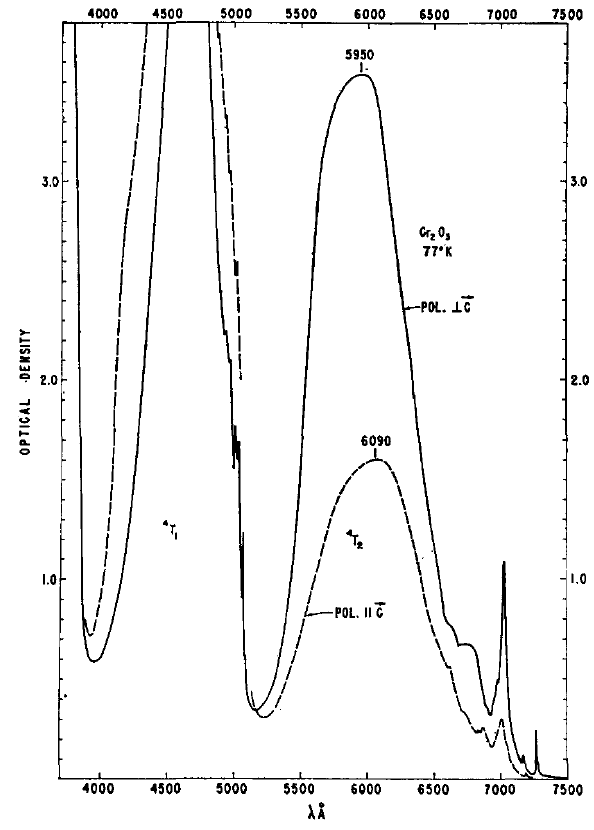
\includegraphics[width=0.4\textwidth]{Cr2O3_absorption_spectra.PNG}
    \caption{Спектр поглощения $\crome$ в области $d$-$d$ переходов. Широкие полосы соответствуют спин-разрешённым переходам $^4\mathrm{A}_2 \to ^4\mathrm{T}_2$ и $^4\mathrm{A}_2 \to ^4\mathrm{T}_1$. Узкие линии  связаны со спин-запрещённым переходом $^4\mathrm{A}_2 \to ^2\mathrm{E}$ \cite{McClure}.}
    \label{fig:cr2o3_absorption}
\end{figure}

Кристалл $\crome$ имеет ромбоэдрическую решётку типа корунда (пространственная группа $R\bar{3}c$) \cite{Sviridov1976, McClure}. При температуре ниже точки Нееля ($T_N = 307.6$ K) в нём устанавливается антиферромагнитный порядок: спины ионов Cr$^{3+}$ (электронная конфигурация $3d^3$) направлены вдоль оси $C_3$ и антипараллельны на соседних ионах   (см. рис \ref{fig:cr2o3_structure}) \cite{Allen1969}. Хотя кристаллическая решётка $\crome$ центросимметрична, антиферромагнитная структура этот центр инверсии не сохраняет \cite{Allen1969}.

\begin{figure}[htbp]
    \centering
    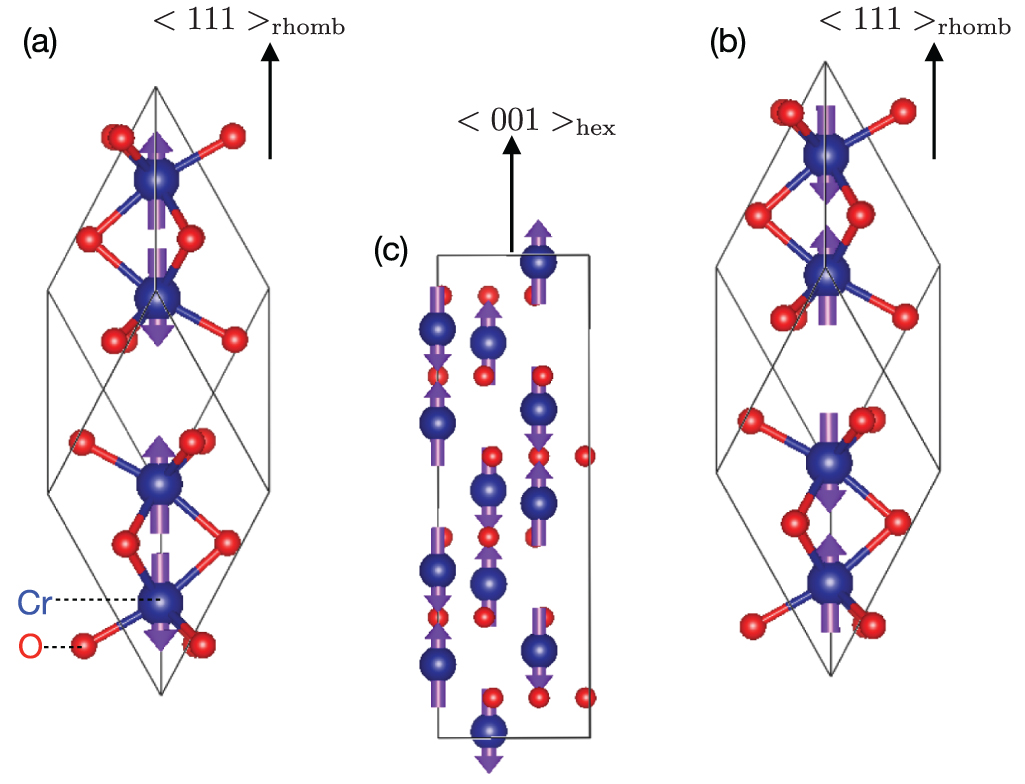
\includegraphics[width=0.6\textwidth]{Cr_scheme.jpg}
    \caption{Кристаллическая структура $\crome$ (тип корунда). Синие сферы $-$ ионы Cr$^{3+}$, красные $-$ ионы O$^{2-}$. Стрелками показано антиферромагнитное упорядочение спинов ионов Cr$^{3+}$ вдоль оси $C_3$ \cite{Bousket_Cr_structure}.}
    \label{fig:cr2o3_structure}
\end{figure}

Ион Cr$^{3+}$ в октаэдрическом кристаллическом поле имеет основное состояние $^4\mathrm{A}_2$ ($L \approx 0$, полный спин $S = 3/2$). Первыми возбуждёнными состояниями являются дублетные термы $^2\mathrm{E}$, $^2\mathrm{T}_1$, $^2\mathrm{T}_2$ ($S = 1/2$) и квартетные термы $^4\mathrm{T}_2$, $^4\mathrm{T}_1$ \cite{Sviridov1976}. В спектре поглощения $\crome$ широкие интенсивные полосы обусловлены спин-разрешёнными переходами $^4\mathrm{A}_2 \to ^4\mathrm{T}_2$ и $^4\mathrm{A}_2 \to ^4\mathrm{T}_1$, тогда как узкие линии в красной области (1.70--1.74 эВ) соответствуют спин-запрещённому переходу $^4\mathrm{A}_2 \to ^2\mathrm{E}$ \cite{McClure, Sviridov1976}.




Возбуждённые состояния в магнитных диэлектриках, таких как $\crome$, принято описывать в терминах экситонов Френкеля \cite{Loudon1968}. В отличие от экситонов Ванье$-$Мотта в полупроводниках, имеющих большой радиус, экситоны Френкеля локализованы на одном или нескольких соседних узлах решётки \cite{Frenkel}. В $\crome$ они образуются из одноионных $d$-$d$ переходов Cr$^{3+}$ за счёт межионного взаимодействия \cite{Allen1969}. Малая ширина экситонных линий в $\crome$ \cite{Allen1969} предполагает большое время жизни, что  благоприятно для таких процессов, как спиновая ориентация.

Элементарная ячейка $\crome$ содержит четыре иона Cr$^{3+}$. Взаимодействие между ними приводит к тому, что вместо четырёх одинаковых одноионных переходов возникают четыре экситонных состояния с разной энергией. Этот эффект называется давыдовским расщеплением \cite{VanderZiel, Allen1969}. В результате из каждого одноионного перехода $^4\mathrm{A}_2 \to ^2\mathrm{E}$ формируется система экситонных уровней, симметрия которых определяется магнитной пространственной группой кристалла \cite{Allen1969}.

Обобщая сказанное, рассмотрим последовательность расщеплений, приводящую к наблюдаемой системе экситонных уровней \cite{Allen1969}. Первый этап $-$ учёт тригонального поля и спин-орбитальной связи (группа симметрии $C_3$). Затем дополнительно расщепляет уровни обменное взаимодействие.  В результате терм $^4\mathrm{A}_2$ расщепляется на четыре уровня $a_6\uparrow$, $a_6\downarrow$, $a_4\uparrow$, $a_5\downarrow$ (стрелка указывает преимущественную проекцию спина $S_z$), а терм $^2\mathrm{E}$ $-$ на четыре уровня $a_4\uparrow$, $a_5\downarrow$, $a_6\uparrow$, $a_6\downarrow$ с обратным порядком спиновых проекций для нижней пары. Наконец, давыдовское расщепление, обусловленное передачей возбуждения между ионами в элементарной ячейке, формирует экситонные состояния, наблюдаемые в спектрах.

Правила отбора получены из  классификации экситонных состояний по неприводимым представлениям точечной группы $D_3$, которая описывает преобразования пространственных координат в низкосимметричной магнитной фазе\cite{Allen1969}. Основное состояние кристалла  преобразуется по представлению $A_1$. Оператор электрического дипольного момента преобразуется по компонентам вектора. Компоненты $E_x, E_y$, ответственные за $\sigma$-поляризацию ($\mathbf{E} \perp C_3$), преобразуются по двумерному представлению $E$. Компонента $E_z$ ($\pi$-поляризация, $\mathbf{E} \parallel C_3$) преобразуется по представлению $A_2$. Применяя правило, согласно которому матричный элемент перехода отличен от нуля, если представление конечного состояния содержится в прямом произведении представлений оператора и начального состояния, получаем правила отбора для электрических дипольных переходов из основного состояния $A_1$. Переходы в состояния, преобразующиеся по представлению $E$, разрешены в $\sigma$-поляризации, так как $E \otimes A_1 = E$. Экспериментально этим переходам соответствуют линии 1 и 4 \cite{Allen1969}. Переходы в состояния, преобразующиеся по представлению $A_2$, разрешены в $\pi$-поляризации ($A_2 \otimes A_1 = A_2$). Им соответствуют линии 2 и 3 \cite{Allen1969}. Переходы в состояния $A_1$ электрически дипольно запрещены, так как $A_1 \otimes A_1 = A_1$ не содержит представлений $E$ или $A_2$ (см. рис. \ref{fig:cr2o3_selection_rules}) \cite{Allen1969, Pavlov}.  Результат данного теоретико-группового анализа согласуется с экспериментом \cite{Allen1969}.

% ВСТАВКА 3: ПРАВИЛА ОТБОРА
\begin{figure}[htbp]
    \centering
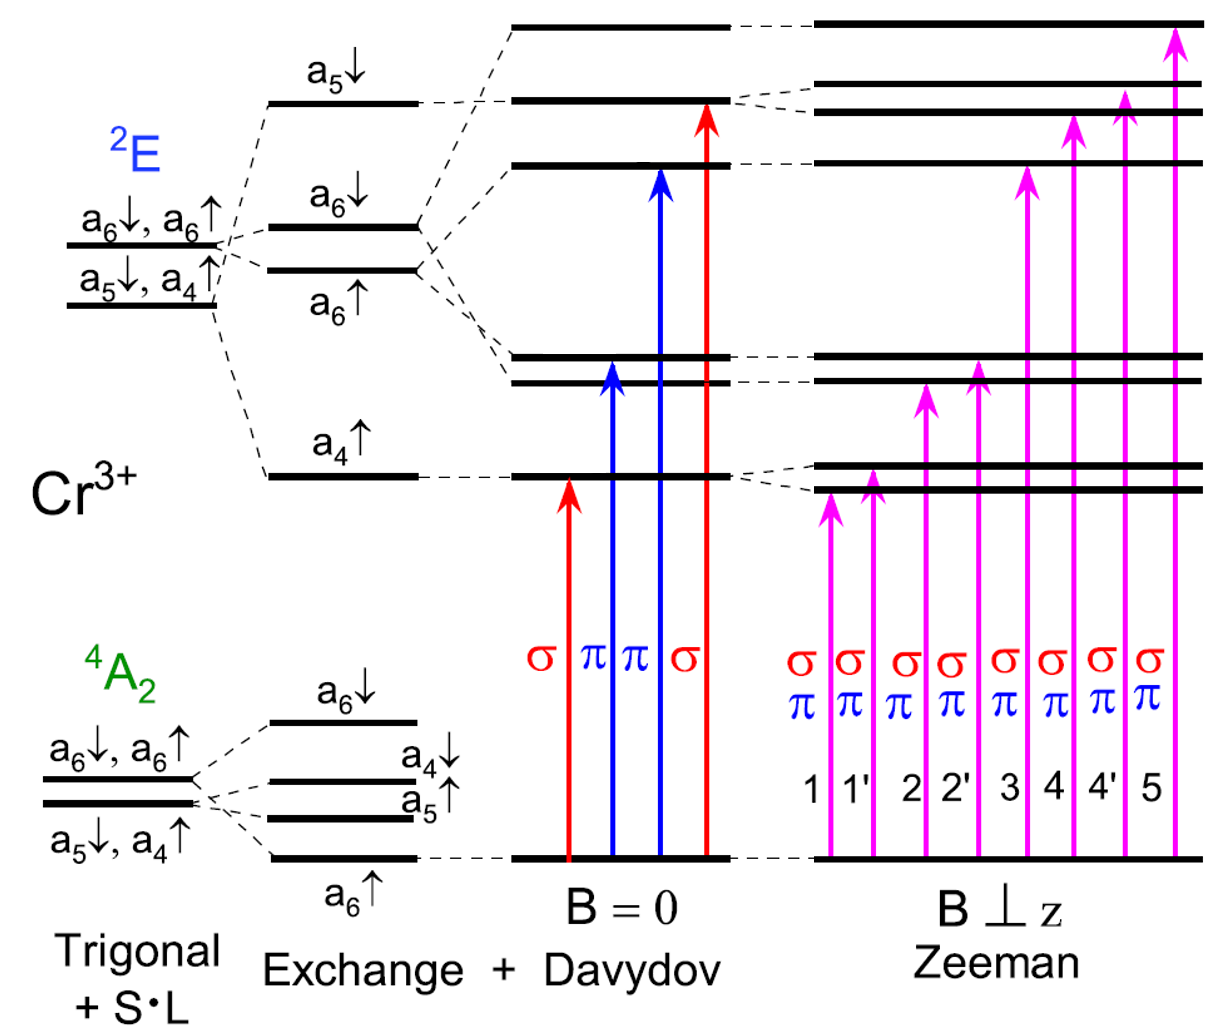
\includegraphics[width=0.7\textwidth]{sel_rules.PNG}

    \caption{Схема правил отбора для электрических дипольных переходов из основного состояния $A_1$ в экситонные состояния $\mathrm{Cr}^{3+}$ \cite{Pavlov}. Состояния $E$ активны в $\sigma$-поляризации ($\mathbf{E} \perp C_3$), состояния $A_2$ --- в $\pi$-поляризации ($\mathbf{E} \parallel C_3$), переходы в $A_1$ запрещены.}
    \label{fig:cr2o3_selection_rules}
\end{figure}

Хотя из-за спин-орбитальной связи и тригонального поля проекция спина $S_z$ не является хорошим квантовым числом, она остаётся почти сохраняющейся величиной \cite{Allen1969}. Это позволяет интерпретировать правила отбора, используя изменение проекции спина $\Delta S_z$, а также даёт предсказания для взаимодействия с циркулярно поляризованным светом. В основном состоянии ($^4\mathrm{A}_2$) ион Cr$^{3+}$ имеет полный спин $S=3/2$. В нижних состояниях возбуждённого дублета $^2\mathrm{E}$ ($a_4\uparrow$ и $a_5\downarrow$) из-за отрицательного $g$-фактора порядок проекций оказывается обратным по сравнению с основным состоянием \cite{Allen1969}. Это означает, что состояние $a_4\uparrow$ (конечное для линии 1) имеет преимущественную проекцию $S_z \approx -1/2$, а состояние $a_5\downarrow$ (конечное для линии 2) имеет преимущественную проекцию $S_z \approx +1/2$. С учётом этой оговорки, правило изменения спина приобретает следующий вид. $\sigma$-переходы (линии 1 и 4) характеризуются изменением $\Delta S_z = \pm 1$ (в проекции на ось $C_3$). Это соответствует классическому дипольному правилу отбора для циркулярно поляризованного света: поглощение фотона с $\sigma^-$ поляризацией ($\Delta S_z = -1$) преимущественно заселяет состояние $a_4\uparrow$ (линия 1), а поглощение с $\sigma^+$ ($\Delta S_z = +1$) — состояние $a_4\downarrow$ (линия 4). $\pi$-переходы (линии 2 и 3) характеризуются изменением $\Delta S_z = 0, \pm 2$ \cite{Allen1969, Pavlov}.  Таким образом, несмотря на примешивание других проекций из-за спин-орбитальной связи, оптическая ориентация спина в $\crome$ подчиняется простому правилу: $\sigma^-$ свет преимущественно генерирует спины $S_z \approx -1/2$, а $\sigma^+$ свет — спины $S_z \approx +1/2$ \cite{Allen1969}.

Рассмотрим теперь эффект приложения магнитного поля в геометрии Фойгта ($\mathbf{B} \perp C_3$). Внешнее поле понижает симметрию системы. Компоненты поля $B_x$ и $B_y$ преобразуются по тому же двумерному представлению $E$, что и компоненты электрического поля для $\sigma$-поляризации. Это означает, что возмущение $\hat{H}_B$ может связывать (смешивать) состояния, принадлежащие разным неприводимым представлениям. В частности, происходит смешивание состояний $E$ и $A_2$, а также $E$ и $A_1$ \cite{Allen1969}. В результате этого смешивания в волновые функции изначально «запрещённых» состояний $A_2$ и $A_1$ добавляется компонента от разрешённых состояний $E$. Как следствие, оптические переходы на эти состояния становятся разрешёнными в $\sigma$-поляризации. Аналогичным образом, благодаря смешиванию, переходы на состояния $E$ могут приобретать $\pi$-поляризацию. Иными словами, в геометрии Фойгта происходит изменение правил отбора, и все переходы становятся активными в обеих поляризациях \cite{Allen1969, Pavlov}. Кроме того, магнитное поле снимает вырождение двумерных представлений $E$, что проявляется в виде зеемановского расщепления линий 1 и 4 на дублеты \cite{Allen1969}. 

\newpage
\section{ХАРАКТЕРИЗАЦИЯ ОБРАЗЦА}
Поскольку для изучения спиновой релаксации планируется использовать методику фемтосекундной магнитооптической накачки-зондирования, необходимо определить оптимальные параметры накачки и зондирующего луча. Для этого и проводилась характеризация образца. В ходе характеризации требовалось установить   положение экситонных линиий соответствующих переходам  $^4A_2 \longrightarrow ^2E$ ионов $\mathrm{Cr}^{3+}$ в пленке $\crome$. Хотя положение  в объемном $\crome$,  хорошо известно, необходимо было проверить, что толщина пленки достаточна для проявления объемных свойств материала. Кроме того, требовалось определить длину волны зондирующего луча, при которой магнитооптический отклик максимален.

Для определения оптимальных параметров возбуждения спиновой ориентации в образце была выбрана методика спектроскопии поглощения, а для определения оптимальных параметров детектирования$ -$ магнитооптическая спектроскопия. Рассмотрим методы и результаты характеризации более подробно.

\subsection{Спектроскопия поглощения}

Коэффициент поглощения, или оптическая плотность ($D$), на заданной длине волны определяется как  десятичный логарифм отношения интенсивности падающего излучения ($I_0$) к интенсивности излучения, прошедшего через образец ($I$):

\begin{equation}
D = lg\left(\frac{I_0}{I}\right) = -lg \left(\frac{I}{I_0}\right)
\end{equation}

На основе рассчитанных значений оптической плотности для каждой длины волны строится спектр поглощения. Нас интересует спектр поглощения, обусловленный переходами $^4A_2 \longrightarrow ^2E$ ионов $\mathrm{Cr}^{3+}$ в АФМ $\crome$. 

Оптическое поглощение в $\crome$ лучше всего описывается в рамках теории френкелевских экситонов \cite{VanderZiel}.
Поскольку образование экситонов связано с поглощением фотонов строго определённой энергии \cite{Piter}, в спектре поглощения ожидается появление узких пиков.

Для изучаемых переходов положение этих линий в спектре известно. Ожидается, что они будут находиться в спектральном диапазоне  $1.7 - 1.8$ эВ \cite{Pavlov}.

Энергия связи экситонов часто сравнима с тепловой энергией при комнатной температуре, что приводит к их термическому размыванию. 
Для наблюдения узких экситонных линий образец необходимо охлаждать. В нашем эксперименте для этого использовался азотный криостат замкнутого цикла. Измерения проводились при температуре $68 K$.

В качестве широкополосного источника излучения использовалась лампа, излучающая в спектральном диапазоне 640 $-$ 820 нм.
Для уменьшения рассеяния и сохранения высокой интенсивности падающего света лампа освещала диафрагму, изображение которой с помощью собирающей линзы проецировалось на образец. 
После образца изображение, с помощью второй собирающей линзы, передавалось в спектрометр. Полная схема установки представлена на рис. \ref{fig:lamp_set_up}.


\begin{figure}[h]
  \centering
    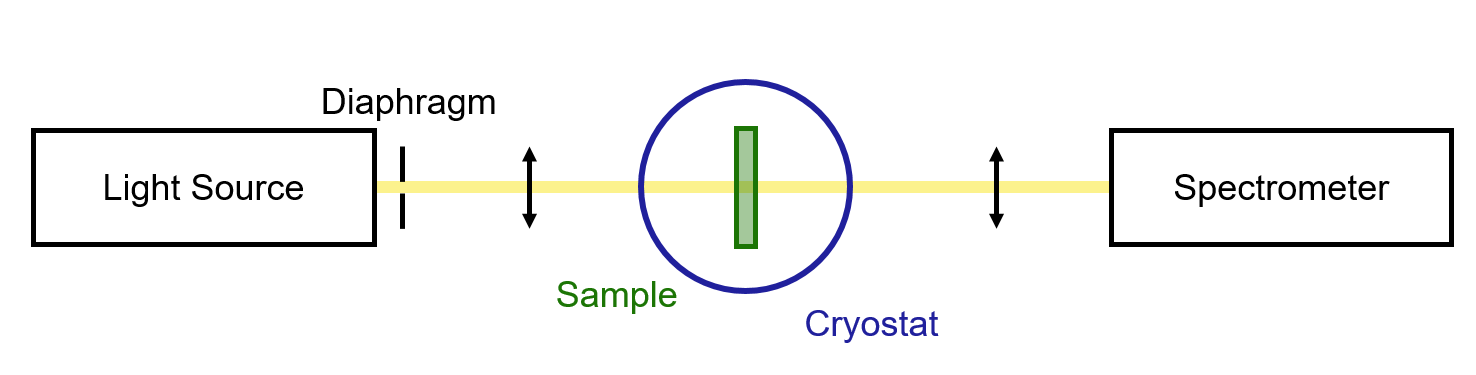
\includegraphics[width=1\linewidth]{set_up_absorption.PNG}
    \caption{Схема установки спектроскопии поглощения}  
    \label{fig:lamp_set_up}
\end{figure}

Сначала измерялся опорный спектр интенсивности падающего излучения (без образца), а затем спектр интенсивности излучения, прошедшего через образец.
Для каждой длины волны, строилось отношение этих величин. Результат представлен на рис. \ref{fig:nm_more_light}.

\begin{figure}[h]
  \centering
    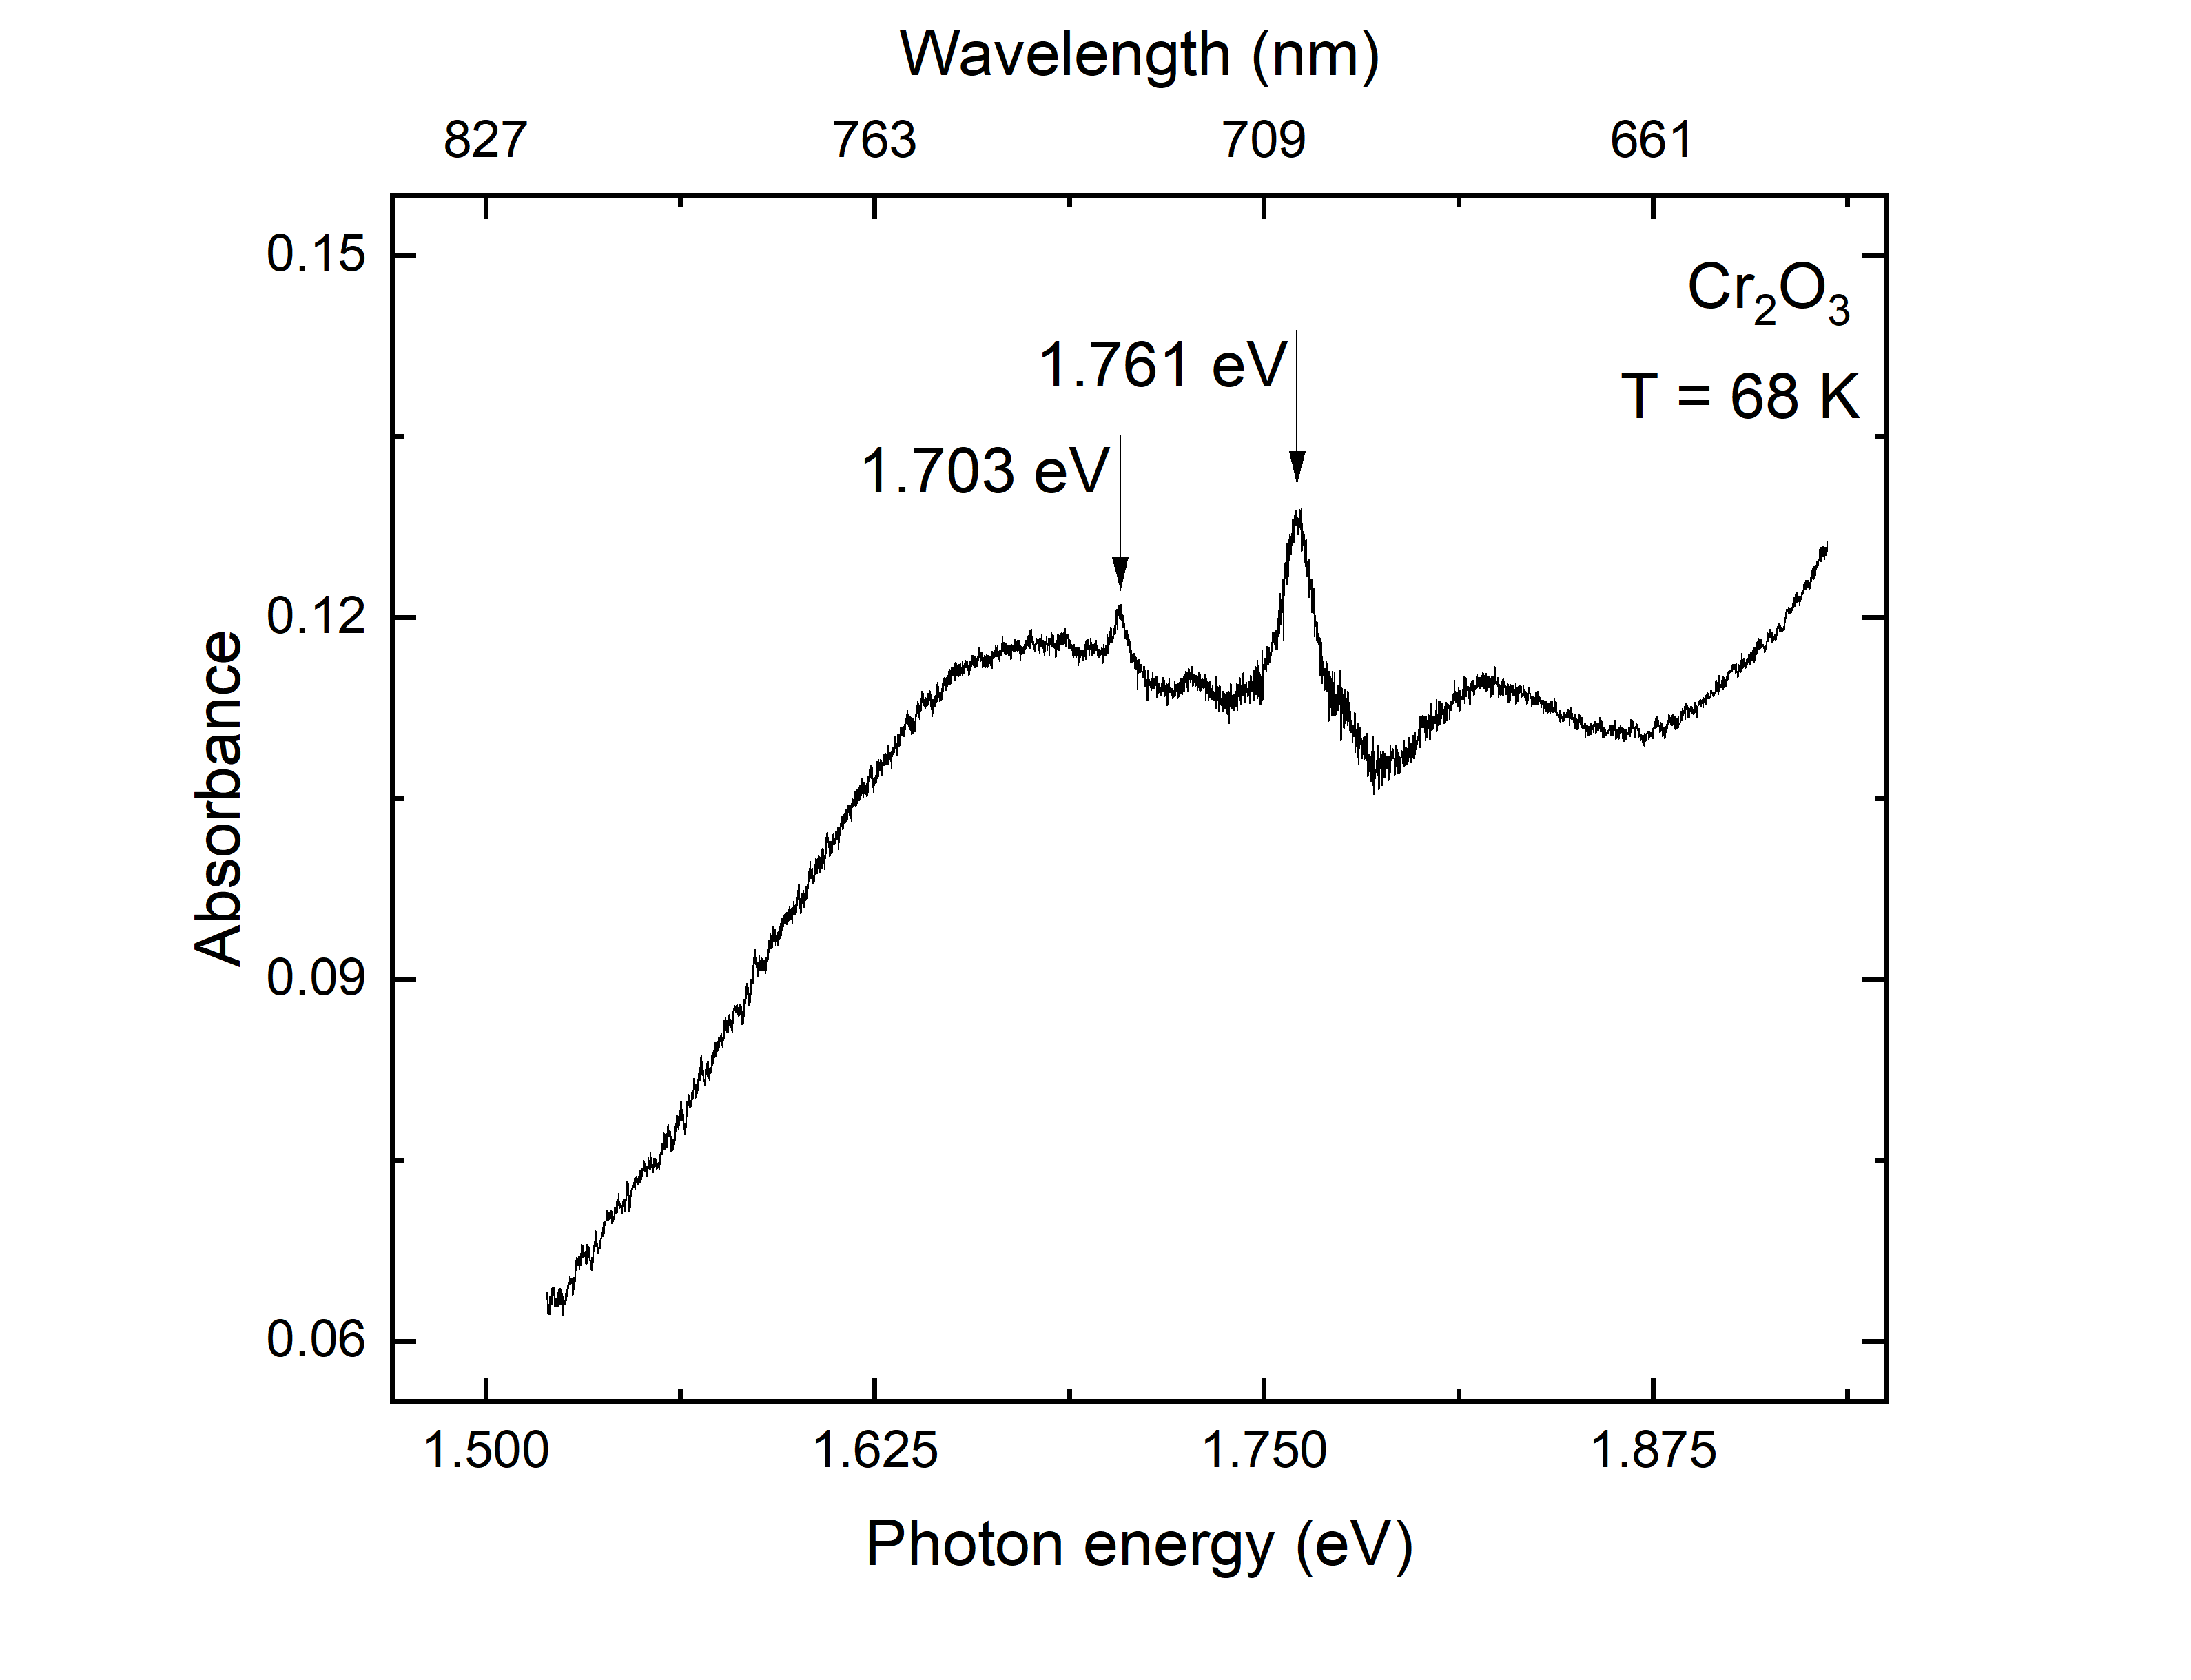
\includegraphics[width=0.8\linewidth]{Absorption_arrows.png}
    \caption{Спектр поглощения пленки $\crome$  при температуре $68K$, наблюдаются линии экситонов на 705нм и 730нм}
    \label{fig:nm_more_light}
\end{figure}

Как и ожидалось, на общем плавном фоне поглощения, возрастающем в длинноволновой области, наблюдаются два резких пика, расположенных  на длинах волн 705 нм и 730 нм.

Чтобы сопоставить полученные данные с литературными \cite{Pavlov}, длины волн, соответствующие линиям были пересчитаны в энергии фотонов. Связь между энергией фотона $E$ (в эВ) и длиной волны $\lambda$ (в нм) описывается приближённой формулой:

\begin{equation}
E_\text{эВ} = \frac{1239.8}{\lambda_\text{нм}}
\end{equation}

Расчёт показывает, что минимумы на отметках 705 нм и 730 нм соответствуют энергиям 1.761 эВ и 1.703 эВ.
Полученные значения хорошо согласуются с указанным в \cite{Pavlov} спектральным диапазоном.

Для резонансного возбуждения спиновой ориентации на экситоне предпочтительно использовать долгоживущие состояния. Так как спектральная ширина линии на 730 нм меньше, чем на 705, для возбуждения целесообразно выбрать именно эту длину волны. 

Отметим также, что положение наблюдаемых пиков  совпадает с таковым в объемном материале.
\subsection{Магнитооптическая спектроскопия}

Для определения оптимальных параметров детектирования спиновой поляризации был выбран метод магнитооптической спектроскопии. Данный метод основан на явлениях эффекта Фарадея и магнитного кругового дихроизма (МКД) \cite{zvezdin_1997}.

При прохождении линейно поляризованного света через намагниченный образец плоскость его поляризации поворачивается. Данное явление называется эффектом Фарадея \cite{zvezdin_1997}. Одновременно возникает разность в поглощении право- и лево-циркулярно поляризованных компонент света, что приводит к появлению эллиптичности. Это явление носит название магнитного кругового дихроизма. Оба эффекта обусловлены тем, что показатели преломления $n_+$ и $n_-$ (а также коэффициенты поглощения) для право- и лево-циркулярно поляризованного света в намагниченной среде становятся различными. Величина этих эффектов пропорциональна намагниченности образца \cite{zvezdin_1997}. 

В данной работе метод магнитооптической спектроскопии использовался для определения спектрального диапазона, в котором магнитооптический отклик образца максимален, и последующего выбора длины волны зондирующего луча. 

Измерения проводились при комнатной температуре в геометрии Фарадея, то есть при распространении света вдоль направления внешнего магнитного поля \cite{zvezdin_1997}. Магнитное поле составляло $B = 1.5$ Тл. Полная схема установки представлена на рис. \ref{fig:magnitoopt_set_up}. 

\begin{figure}[h]
  \centering
    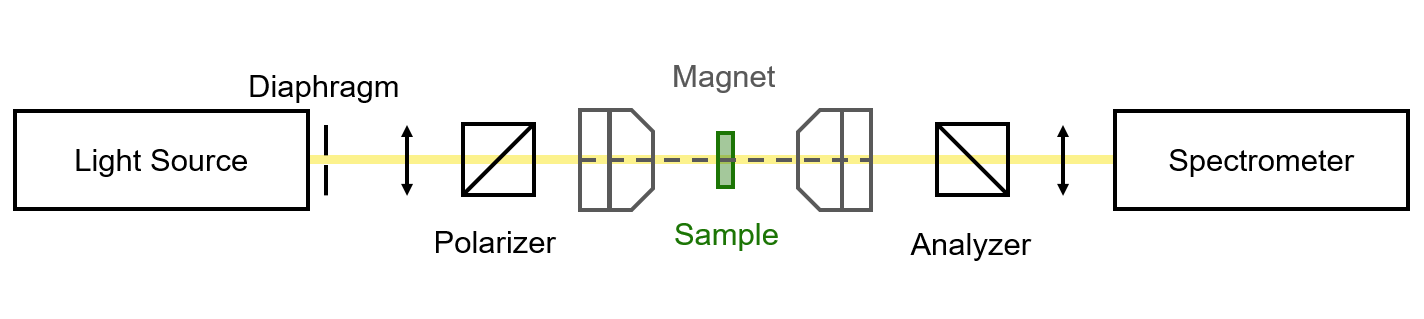
\includegraphics[width=1\linewidth]{set_up_magnetoopt_spectroscopy.PNG}
    \caption{Схема установки магнитооптической спектроскопии}  
    \label{fig:magnitoopt_set_up}
\end{figure}

Зависимость магнитооптического контраста от энергии фотонов представлена на рис. \ref{fig:magnitoopt_result}.

\begin{figure}[h]
  \centering
    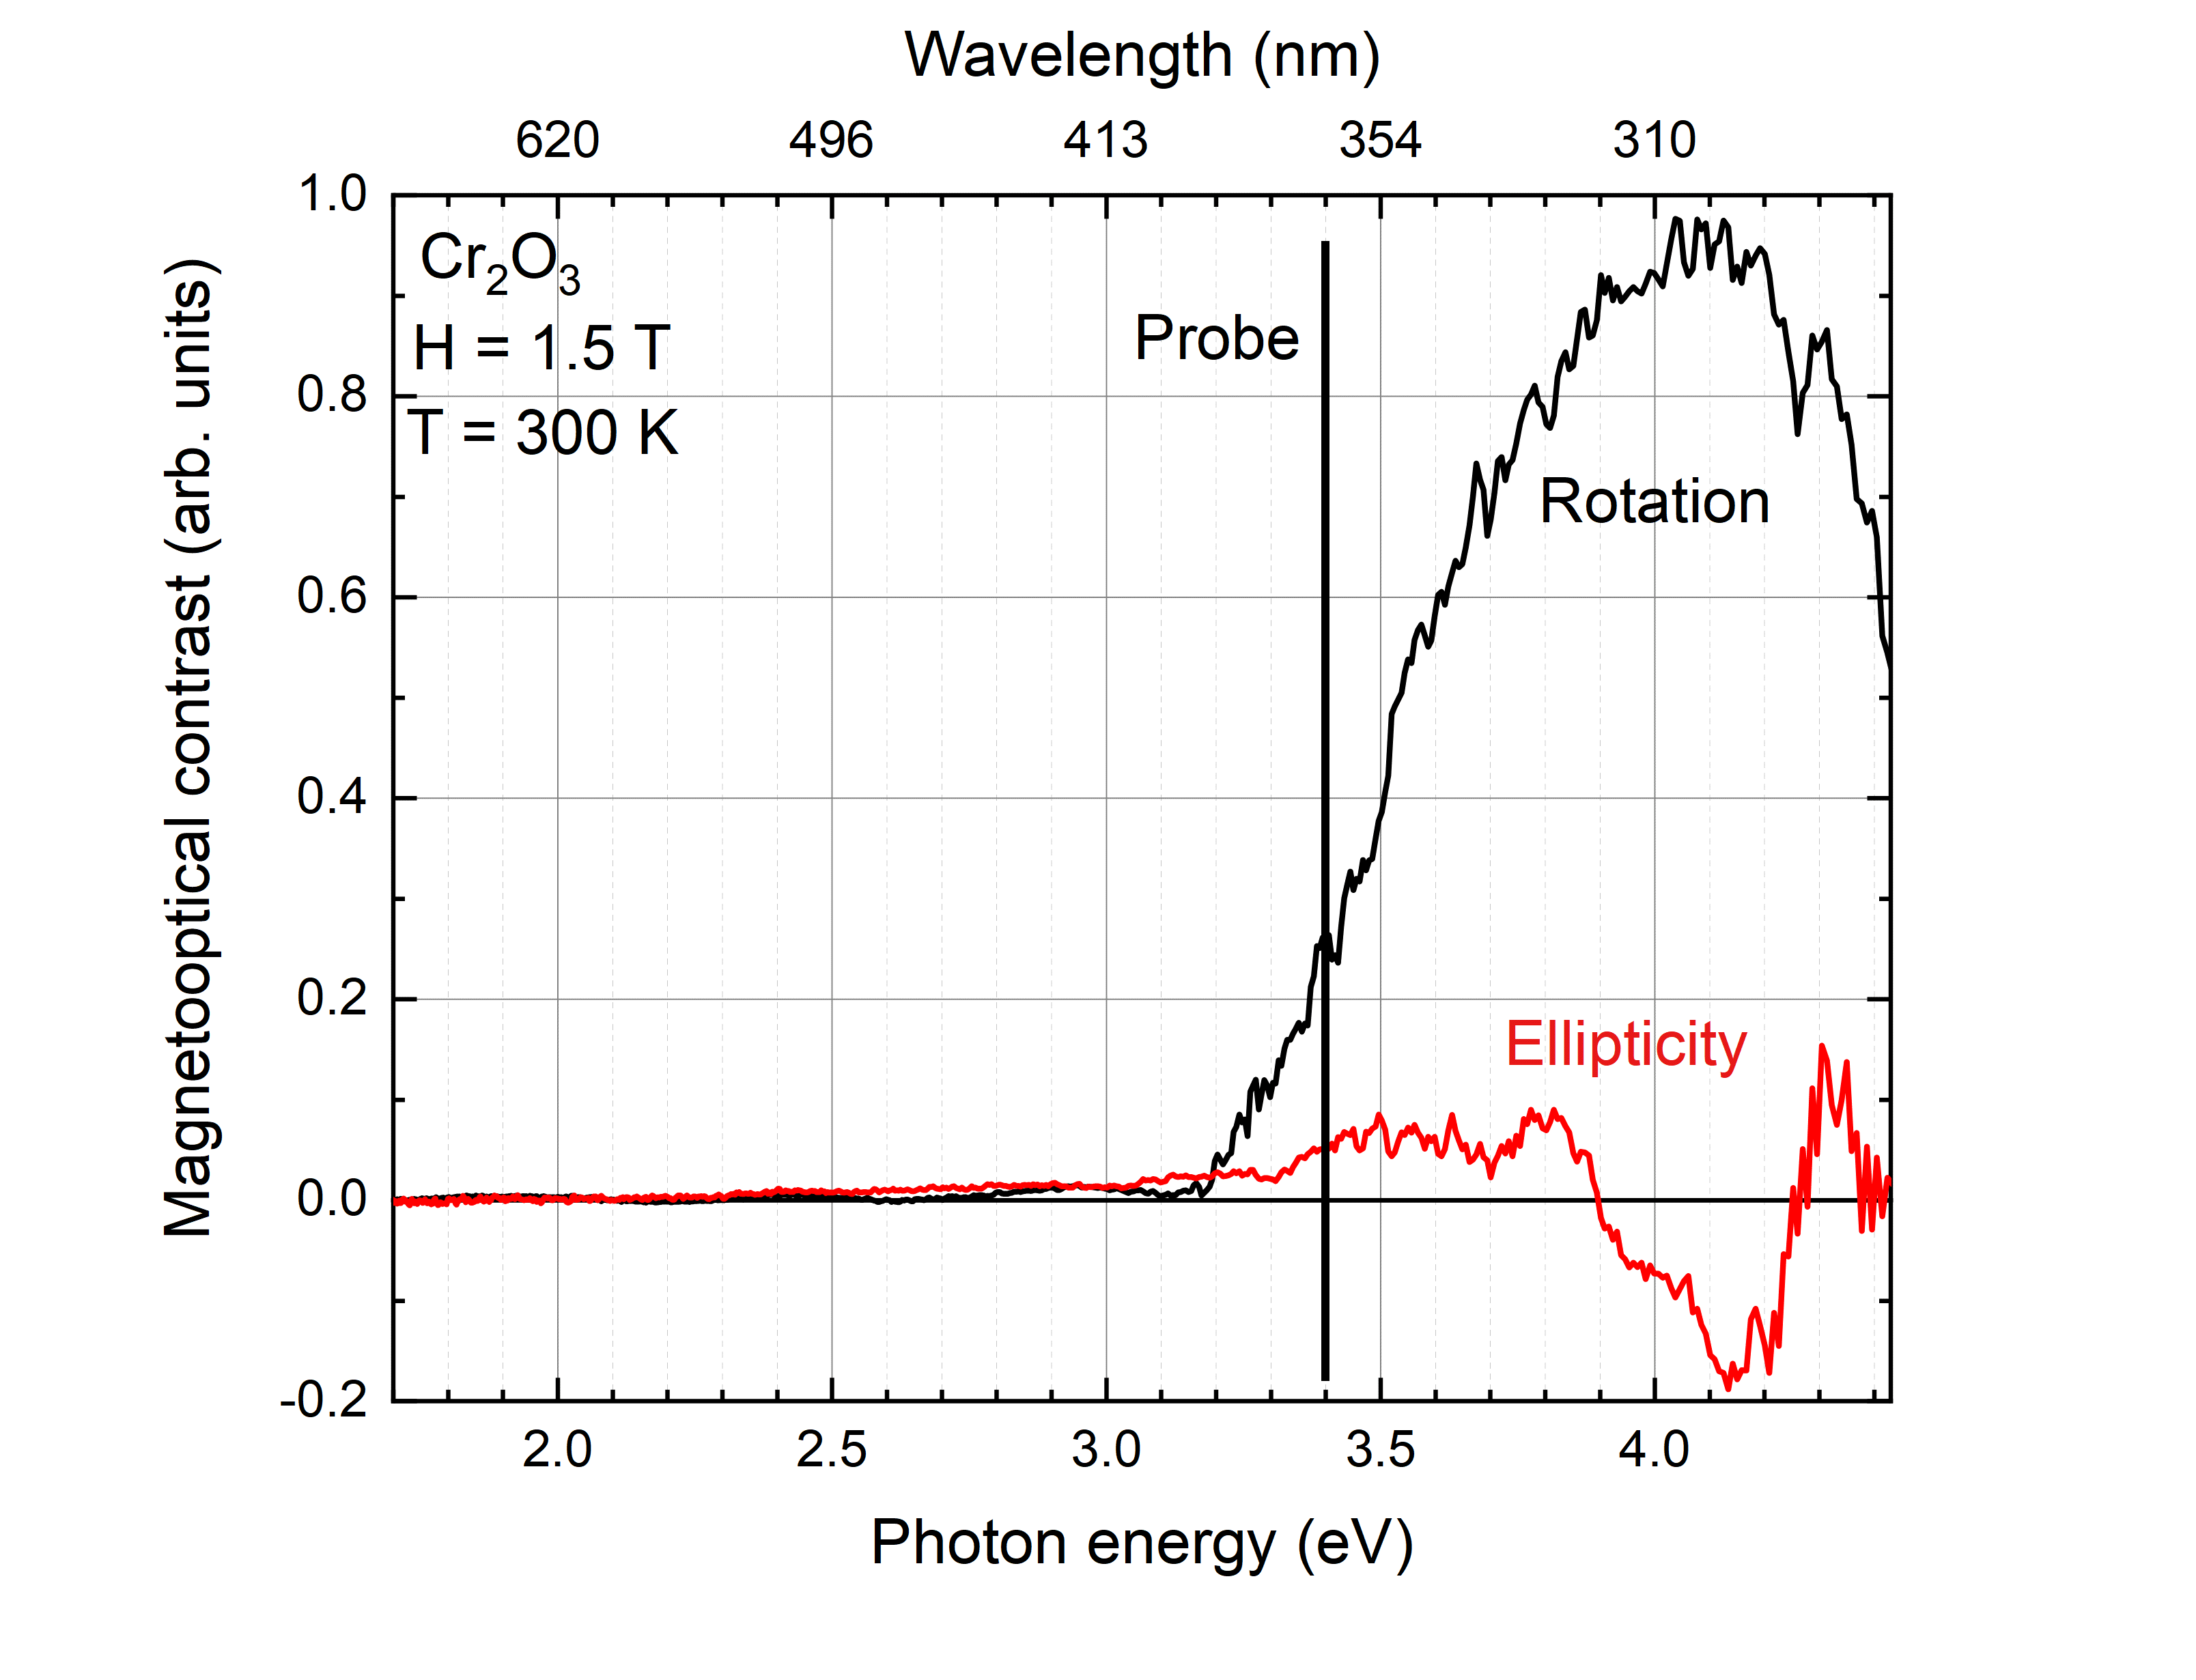
\includegraphics[width=0.8\linewidth]{magnitoopt_spectra_with_probe.png}
    \caption{Зависимость магнитооптического контраста (поворота плоскости поляризации и эллиптичности) от энергии фотонов}  
    \label{fig:magnitoopt_result}
\end{figure}

Согласно представленным на рис. \ref{fig:magnitoopt_result} данным, как поворот плоскости поляризации, так и эллиптичность достигают наибольших значений в коротковолновой части спектра. В связи с этим в качестве зондирующего луча в дальнейших экспериментах по фемтосекундной накачке-зондированию целесообразно использовать вторую оптическую гармонику излучения накачки. Для исследуемого образца данная длина волны соответствует 365 нм (3.397 эВ).




\newpage
\section{ФЕМТОСЕКУНДНАЯ МАГНИТООПТИЧЕСКАЯ НАКАЧКА-ЗОНДИРОВАНИЕ}

Для изучения динамики спиновой поляризации в образце выбрана методика двухцветной оптической фемтосекундной накачки-зондирования с временным разрешением.

Принцип метода заключается в следующем. Мощный фемтосекундный лазерный импульс (накачка) возбуждает динамику намагниченности в среде. Затем в ту же область образца с контролируемой временной задержкой попадает слабый линейно поляризованный импульс (зондирование). Магнитооптические эффекты — вращение плоскости поляризации или появление эллиптичности — пропорциональны проекции намагниченности на волновой вектор зондирующего излучения. Изменяя временную задержку между импульсами накачки и зондирования, можно отслеживать эволюцию намагниченности непосредственно после лазерного возбуждения. Временное разрешение метода определяется длительностью зондирующего импульса (в данном случае $ \sim60$ фс), что позволяет исследовать процессы с субпикосекундным разрешением.

В данной работе использовалась двухцветная схема, которая позволяет исключить влияние рассеянных импульсов накачки на детектирующую систему, а также использовать необходимые спектральные диапазоны для оптимального режима оптического воздействия и детектирования. Поскольку образец представляет собой прозрачную пленку толщиной 500 нм, динамика намагниченности отслеживалась по изменению эллиптичности света в эффекте Фарадея.

Полная схема установки представлена на рис. \ref{fig:exp_set_up}.

\begin{figure}[h]
  \centering
    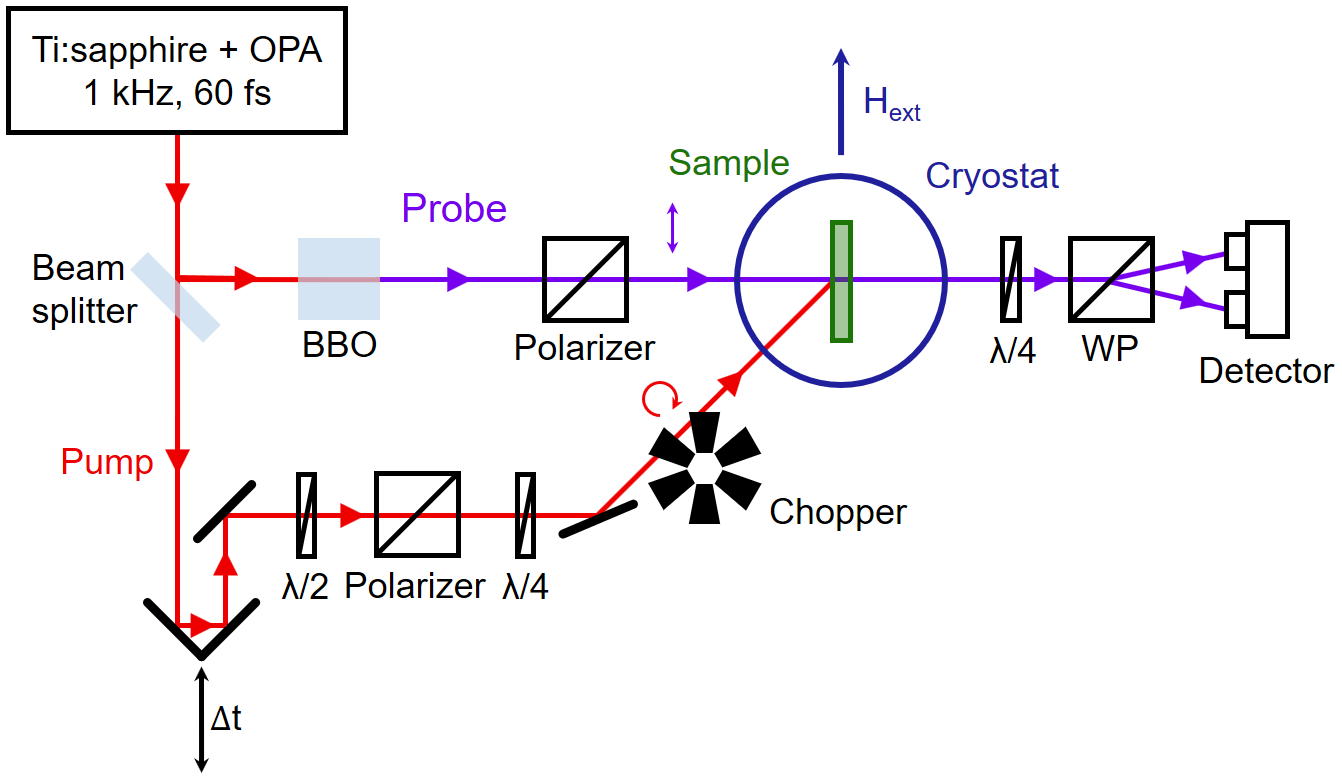
\includegraphics[width=1\linewidth]{set_up_pump_probe_final.PNG}
    \caption{Схема экспериментальной установки магнитооптической фемтосекундной накачки-зондирования с временным разрешением}  
    \label{fig:exp_set_up}
\end{figure}

Источником лазерных импульсов служила лазерная система производства Avesta Project LTD. Фемтосекундный усилитель с рабочим телом Ti:sapphire, длительностью импульса $\sim 40$ фс, частотой повторения 1 кГц и центральной длиной волны 800 нм накачивал оптический параметрический усилитель, что обеспечивало возможность перестройки длины волны в диапазоне от 480 до 4000 нм. В эксперименте для резонансного возбуждения экситонов центральная длина волны накачки составляла 730 нм (1,703 эВ), а нерезонансная $-$ 750 нм (1,653 эВ). Частота зондирующих импульсов соответствовала второй оптической гармонике частоты накачки: 365 нм (3,397 эВ) и 375 нм (3,306 эВ) в резонансном и нерезонансном случае, соответственно. Длительность импульсов накачки и зонда составляла $\sim 60$ фс, спектральная ширина импульсов на полувысоте $\sim 13$ нм (0,03 эВ). Плотность накачки $-$ 130 мДж/см$^2$. Соотношение плотностей накачки между импульсами накачки и зонда было выбрано 100:1. Импульс накачки фокусировался на образце в пятно диаметром около 100 мкм, а пятно зондирующего луча было в два раза меньше. Волновой вектор луча накачки был перпендикулярен поверхности образца.

Для генерации второй оптической гармоники использовался нелинейный кристалл бета-бората бария. После него для подавления первой гармоники и формирования линейной поляризации зондирующего луча были установлены поляризатор и фильтр. Для контроля плотности накачки в луч накачки последовательно помещались пластинка $\lambda/2$ и поляризатор, а для получения требуемой поляризации после них размещалась пластинка $\lambda/4$. Импульсы накачки и зондирования фокусировались на поверхность образца с помощью линз. Задержка между импульсами накачки и зондирования осуществлялась изменением длины оптического пути импульса накачки с помощью оптической линии задержки с установленным на ней ретрорефлектором. Луч накачки модулировался оптомеханическим модулятором на частоте 500 Гц.

Образец помещался в гелиевый криостат замкнутого цикла, позволяющий проводить измерения в температурном диапазоне от 3 K до 300 K. Использование сверхпроводящего магнита дало возможность варьировать магнитное поле в диапазоне от $-$6,5 T до 6,5 T. Измерения проводились в геометрии Фойгта (волновой вектор перпендикулярен индукции внешнего магнитного поля). 

Для детектирования изменения эллиптичности зондирующего луча применялась балансная схема. Пластинка $\lambda/4$ преобразовывала эллиптичность прошедшего через образец пучка в поворот плоскости поляризации. Установленная после неё призма Волластона пространственно разделяла пучок на две компоненты с ортогональными линейными поляризациями, интенсивности которых регистрировались двумя фотодиодами. Сигнал с фотодиодов вычитался с помощью балансного детектора, после чего измерялся на частоте 500 Гц с использованием синхронного усилителя (lock‑in), где происходила демодуляция. Итоговый сигнал усреднялся по большому числу событий.
\newpage

\section{РЕЗУЛЬТАТЫ}
Для подтверждения эффекта оптической ориентации и установления его связи с френкелевскими экситонами в $\crome$ измерения  проводились в двух режимах: резонансном и нерезонансном. Параметры возбуждения выбирались на основании данных характеризации образца.

В резонансном режиме центральная длина волны импульса накачки составляла $\lambda_{\text{pump}} = 730$~нм ($E_{\text{pump}} \approx 1.703$~эВ), что соответствует спин-запрещённому переходу $^4A_2 \rightarrow ^2E$ иона Cr$^{3+}$ с $a_6 \uparrow \rightarrow a_4 \uparrow$ (см. рис.~\ref{fig:exp_points}). Импульс зондирования, генерировавшийся как вторая оптическая гармоника накачки  имел длину волны $\lambda_{\text{probe}} = 365$~нм ($E_{\text{probe}} \approx 3.397$~эВ). В нерезонансном режиме накачка осуществлялась на длине волны $\lambda_{\text{pump}} = 750$~нм ($E_{\text{pump}} \approx 1.653$~эВ) ( см. рис.~\ref{fig:exp_points}). 

\begin{figure}[h]
  \centering
    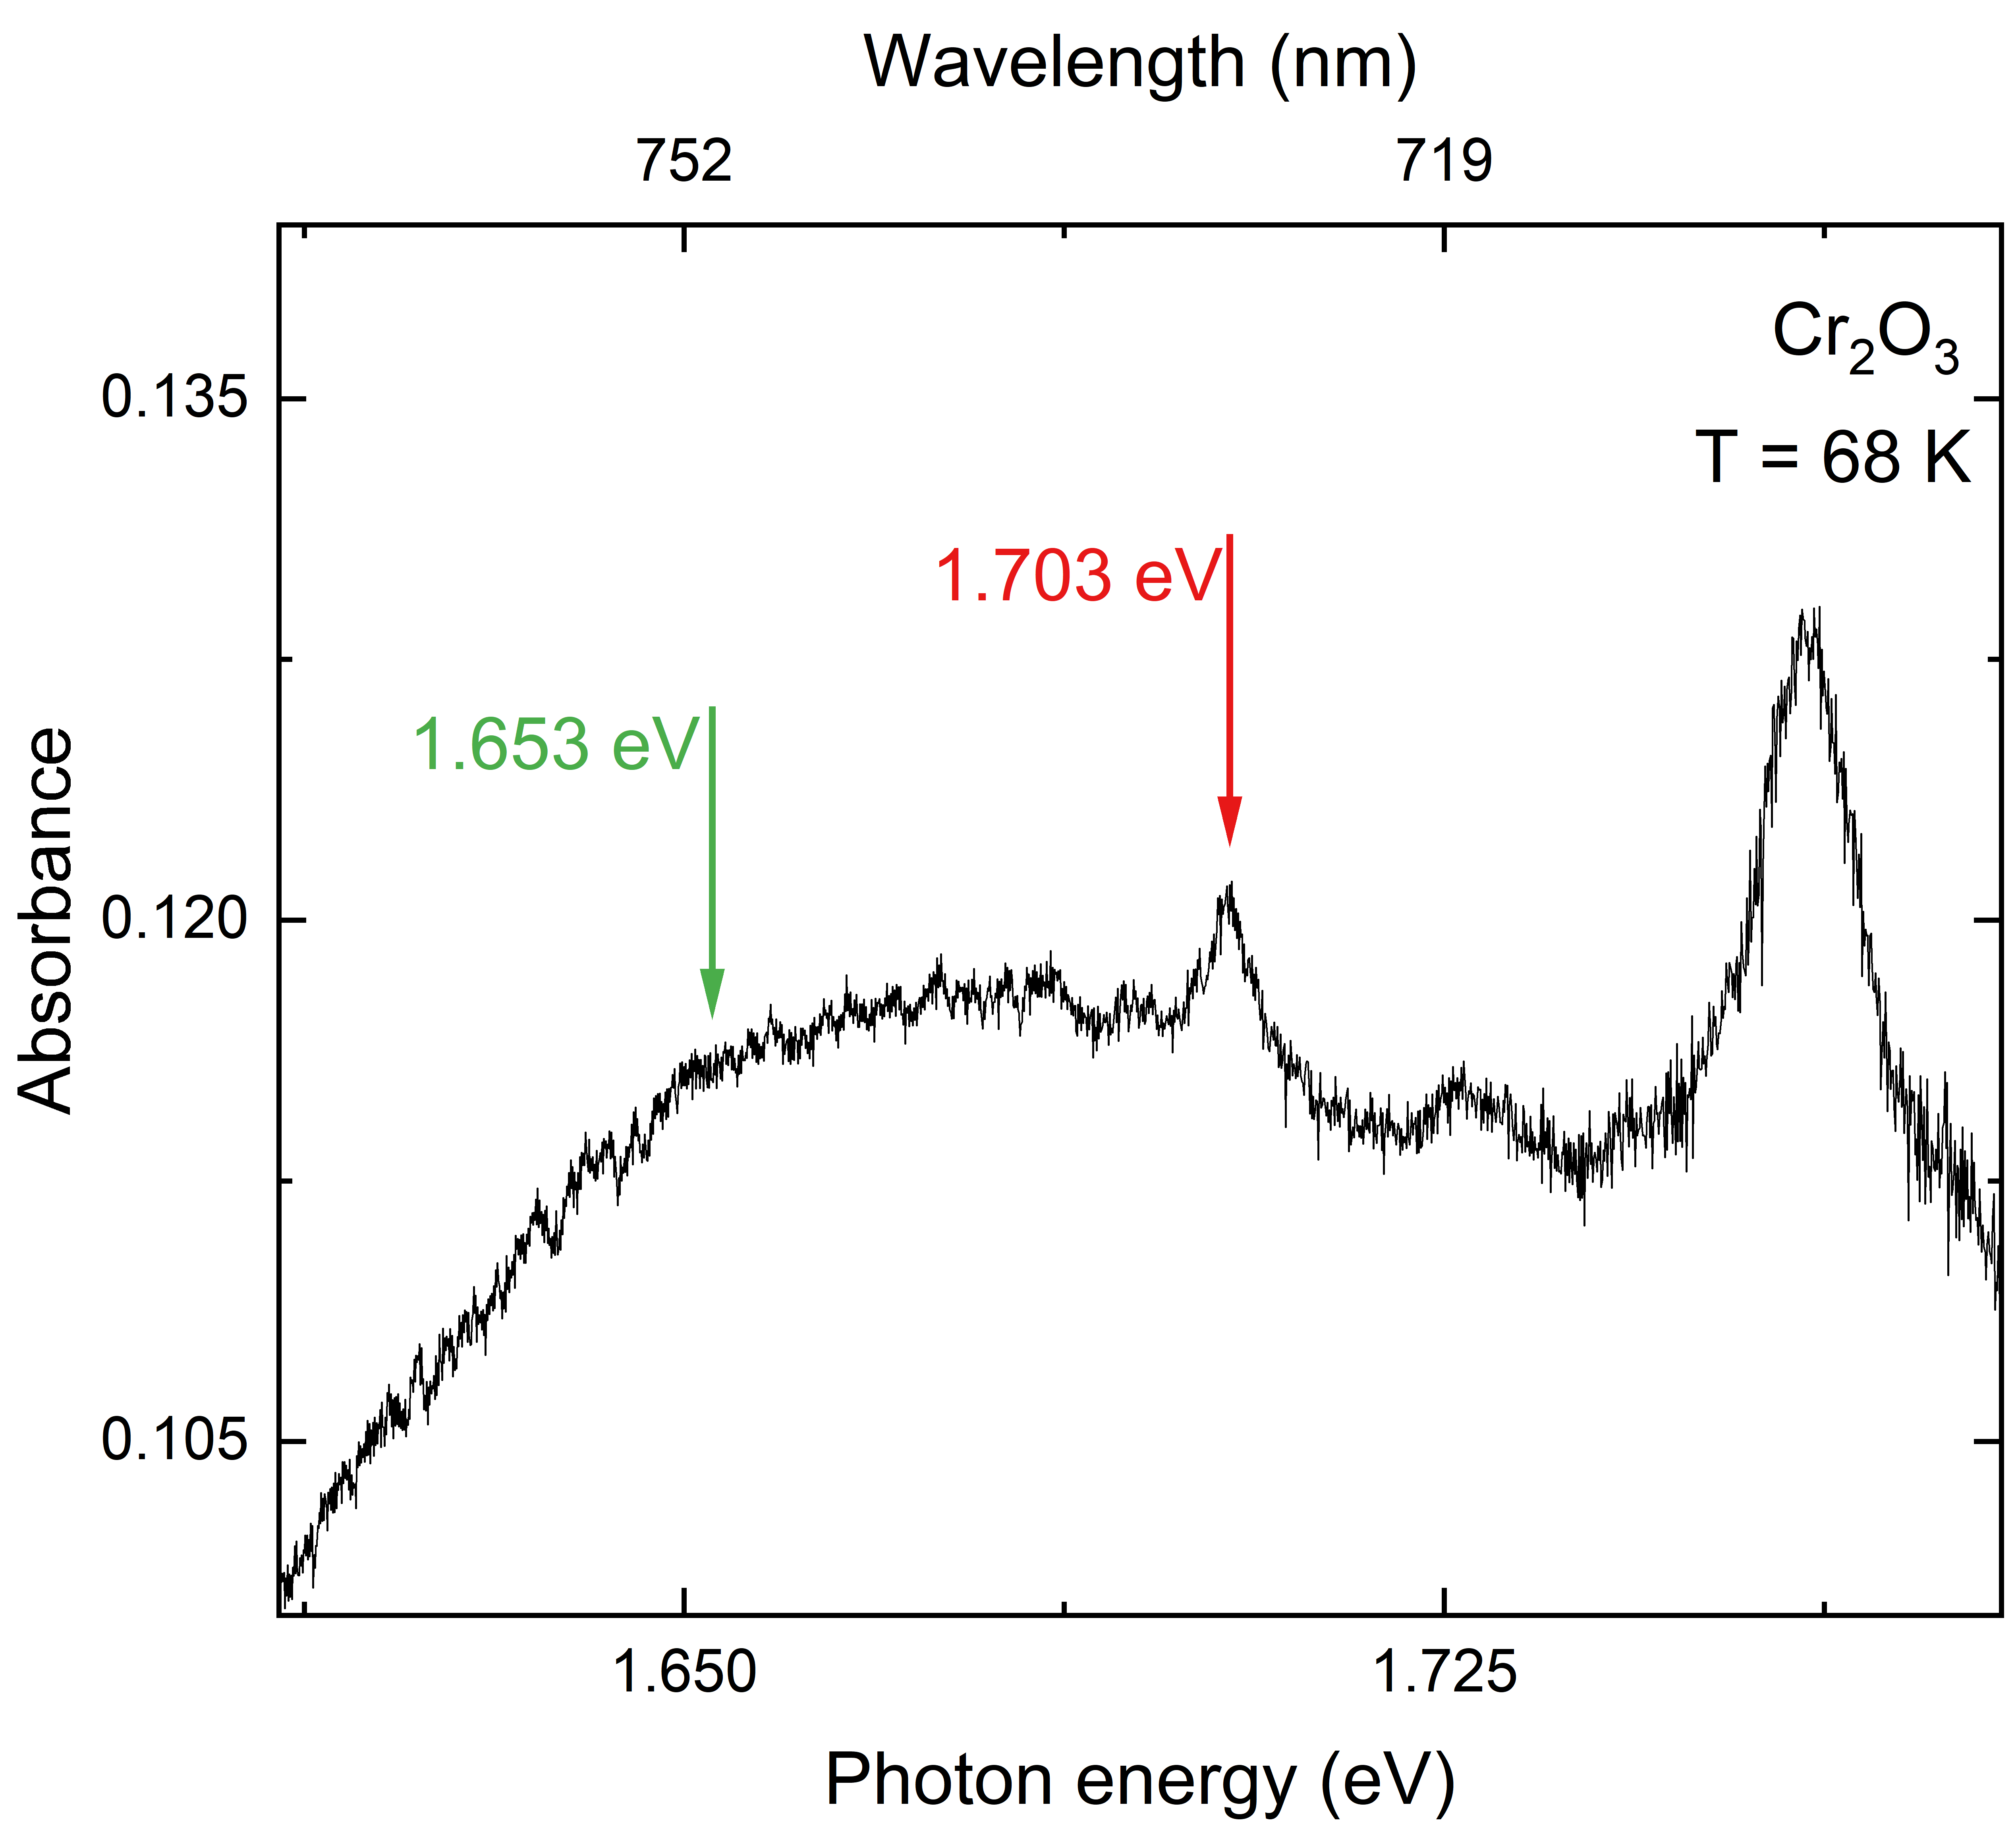
\includegraphics[width=0.5\linewidth]{graph_final.png}
    \caption{Спектр поглощения плёнки $\crome$ при температуре $T = 68$~K. Вертикальными стрелками указаны центральные длины волн и энергии возбуждения в резонансном ($\lambda = 730$~нм, $E = 1.703$~эВ) и нерезонансном ($\lambda = 750$~нм, $E = 1.653$~эВ) режимах. }  
    \label{fig:exp_points}
\end{figure}

На рис.~\ref{fig:results} представлены  зависимости эллиптичности зондирующего луча от времени  для $\sigma^+$ и $\sigma^-$ поляризаций накачки в резонансном и нерезонансном режимах.

Во всех случаях длительность сигнала превышает длительность лазерного импульса ($\sim60$~фс). Это указывает на релаксационный процесс в электронной подсистеме кристалла, а не на мгновенный когерентный отклик. В резонансном режиме характерное время затухания сигнала составило $\sim 1$ пс. В нерезонансном режиме сигнал затухает быстрее.

Более медленная релаксация сигнала в резонансном режиме по сравнению с нерезонансным указывает на возбуждение долгоживущего состояния. Совпадение энергии накачки с экситонным переходом $^4A_2
\rightarrow {}^2E$ позволяет связать этот сигнал с заселенностью экситона.

\begin{figure}[h]
\begin{minipage}[h]{0.5\linewidth}
\center{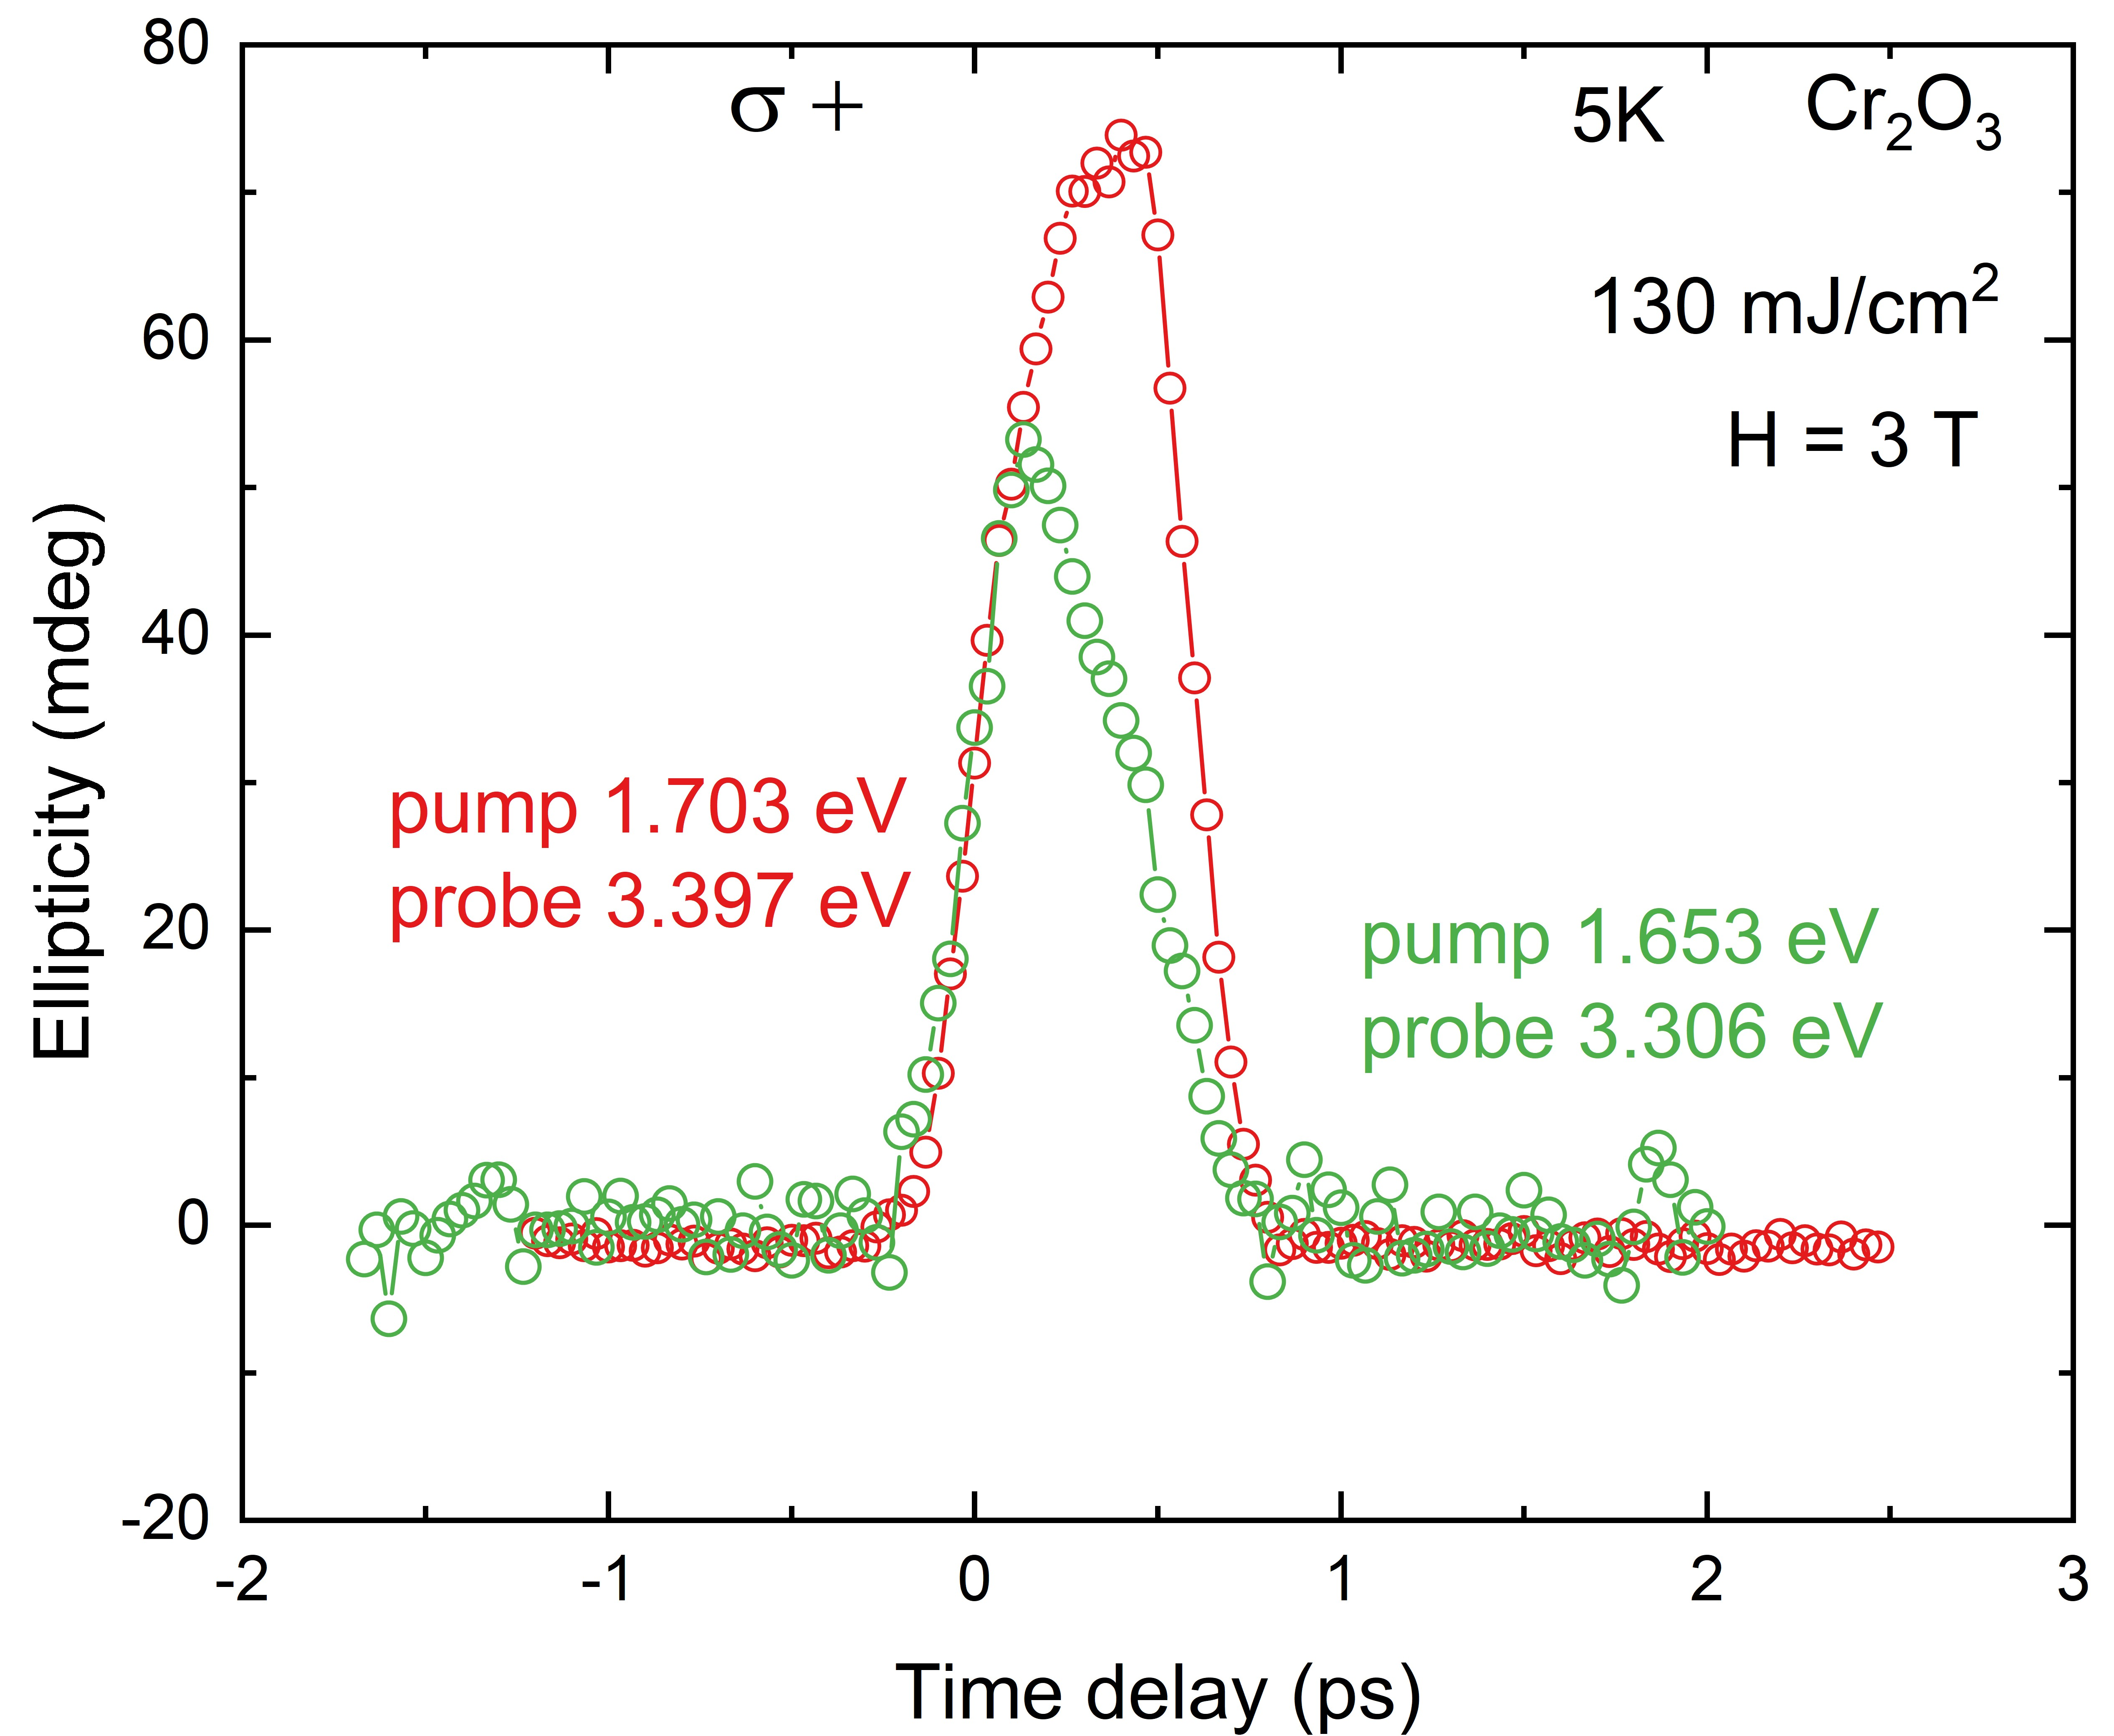
\includegraphics[width=1\linewidth]{730_750_sigm+_final.jpg}} a) \\
\end{minipage}
\hfill
\begin{minipage}[h]{0.5\linewidth}
\center{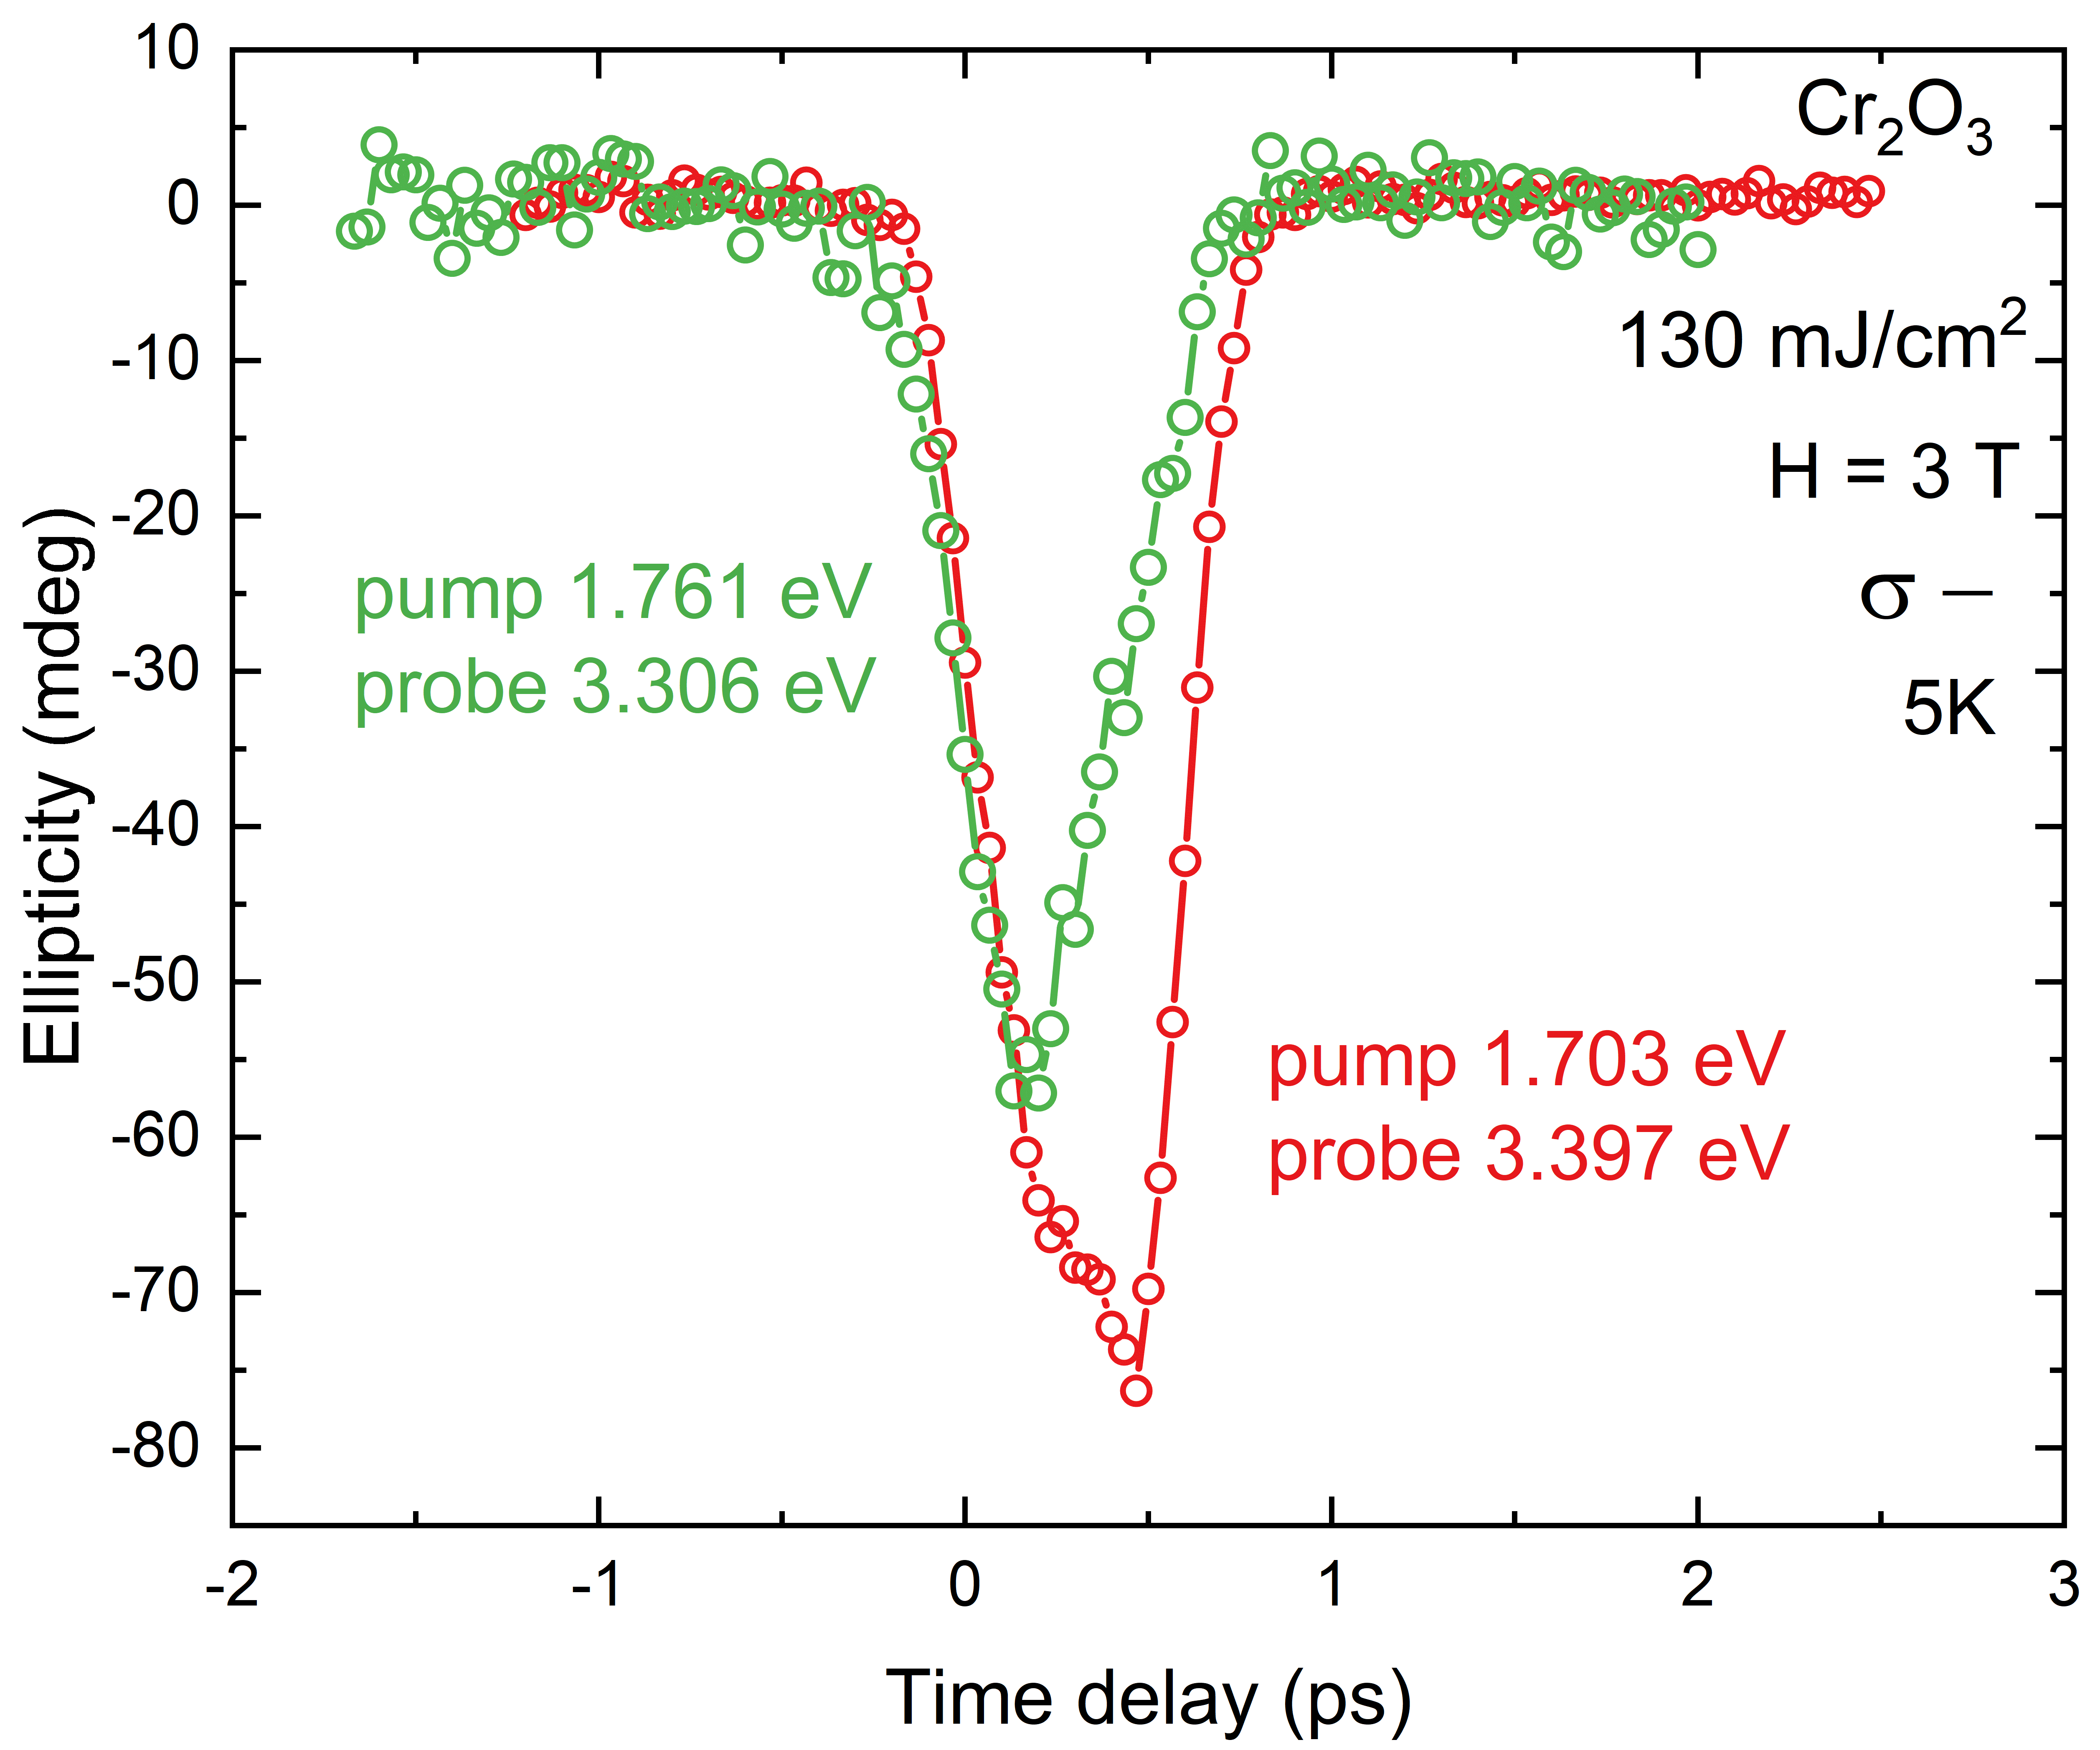
\includegraphics[width=1\linewidth]{sig-_final.png}} b) \\
\end{minipage}
\vfill
 \caption{Временная зависимость эллиптичности зондирующего излучения для резонансного (красная кривая) и  нерезонансного (зеленая кривая) режимов при возбуждении импульсами накачки с а) $\sigma^+$,  и $\sigma^-$,  поляризациями.}
    \label{fig:results}

\end{figure}

О наличии оптической ориентации можно судить по поведению сигнала
при изменении поляризации накачки. Как видно из рис.~\ref{fig:results},
смена поляризации возбуждающего импульса с $\sigma^+$ на $\sigma^-$ приводит
к инверсии знака эллиптичности зондирующего сигнала.

Отсутствие инверсии при смене поляризации было бы характерно для неспиновых
механизмов, в частности, для теплового отклика, вызванного релаксацией
фотовозбуждённых носителей. Наблюдаемая же  инверсия противоречит
тепловому механизму как основной причине сигнала. Дополнительным аргументом служит узость экситонных линий в спектре поглощения (рис.~\ref{fig:cr2o3_absorption}). Из-за узости в линию поглощается лишь малая доля энергии импульса накачки. Соответственно, тепловой вклад, обусловленный релаксацией поглощённой энергии, должен быть незначительным. 
\newpage
\section*{ЗАКЛЮЧЕНИЕ}
\addcontentsline{toc}{section}{ЗАКЛЮЧЕНИЕ}

В работе впервые экспериментально продемонстрирован эффект оптической
спиновой ориентации в диэлектрическом антиферромагнетике Cr$_2$O$_3$
на экситонах Френкеля, возникающих при внутрицентровых $d$-$d$ переходах
ионов Cr$^{3+}$.

В ходе выполнения работы была проведена характеризация плёнки Cr$_2$O$_3$,
в результате которой определены оптимальные параметры возбуждения
(длина волны накачки $\lambda = 730$~нм, соответствующая экситонному
переходу $^4A_2 \rightarrow {}^2E$) и детектирования ($\lambda = 365$~нм).
Создана экспериментальная установка двухцветной фемтосекундной
магнитооптической спектроскопии накачки-зондирования, позволившая
измерять динамику спиновой поляризации с субпикосекундным временным
разрешением.

Измерена временная эволюция магнитооптического сигнала при резонансном
($\lambda_{\text{pump}} = 730$~нм) и нерезонансном ($\lambda_{\text{pump}} = 750$~нм)
возбуждении. Показано, что характерное время затухания сигнала в резонансном
режиме составляет $\sim1$~пс, что существенно превышает время релаксации
в нерезонансном случае. Установлено, что смена поляризации накачки
с $\sigma^+$ на $\sigma^-$ приводит к инверсии знака эллиптичности
зондирующего сигнала, что свидетельствует о спиновой природе наблюдаемого
отклика. Тепловые вклады исключены на основании инверсии сигнала при смене
поляризации накачки и узости экситонных линий, приводящей к малому поглощению
энергии.

Основные результаты работы были представлены в виде устных докладов на:
\begin{itemize}
    \item III Зимней Всероссийской студенческой физико-математической
          конкурсе-школе им. И.Е. Тамма (г. Саров, 26--30 января 2026 г.);
    \item студенческой конференции Алферовского университета (19 мая 2026 г.).
\end{itemize}











\newpage

\section*{СПИСОК ИСПОЛЬЗОВАННЫХ ИСТОЧНИКОВ}
\addcontentsline{toc}{section}{СПИСОК ИСПОЛЬЗОВАННЫХ ИСТОЧНИКОВ}
\printbibliography[heading=none]

\end{document}



• Титульный лист. 
• Задание по выполнению ВКР. 
• Оглавление - перечень названий всех глав, подпунктов, глоссарий (при наличии), список использованных источников, приложения, которые указываются в строгой последовательности с обозначением страниц начала каждой части. 
• Введение - раскрывает актуальность проблемы исследования, цель, задачи, объект, предмет и методы исследования и т.д. 
• Основная часть – состоит, как правило, из соразмерных по объему глав, содержание которых определено РПД/программой ИГА по соответствующим ОПОП: 
- 3 главы - для дипломной работы  бакалавров и магистерской диссертации. 
• Заключение - содержит краткую трактовку полученных результатов, их научную и практическую ценность. 
• Глоссарий (список терминов) - не является обязательной частью. 
• Список использованных источников. 
• Каждая структурная часть ВКР оформляется с новой страницы. Наименования структурных частей в тексте ВКР («ОГЛАВЛЕНИЕ», «ВВЕДЕНИЕ», «ГЛАВА», «ЗАКЛЮЧЕНИЕ», «СПИСОК ИСПОЛЬЗОВАННЫХ ИСТОЧНИКОВ», «ГЛОССАРИЙ») печатаются прописными (заглавными) буквами по центру строки, без подчеркивания. Точка в конце наименования не ставится. 
